
\label{sec:gbb-eventselection}

The overall event selection strategy aims to enhance the purity of gluon splitting to $b \bar b$ events. The gluon splitting process dominates at low $\Delta R$. To isolate this process, we require events to have one $R=1.0$ jet, which is the proxy of the gluon. The $R=1.0$ jet is required to have at least two ghost associated $R=0.2$ track jets, which are proxies of the splitting products of the gluon. The leading track jet is then $b$-tagged. 

The un-prescaled HLT item \textbf{HLT\_j420\_a10\_lcw\_L1J100} triggers on events which have $R=1.0$ jets. The leading $R=1.0$ jet is required to have $p_T>450$ GeV to be on the trigger efficiency pleateu. 

The detailed event selection goes as the following:
\begin{enumerate}
	\item MC events are subject to event cleaning: the average $p_T$ of leading two $R=0.4$ reco jets is less than 1.4 times the $p_T$ of the leading $R=0.4$ truth jet. 
	\item Pass the $R=1.0$ single jet trigger: \textbf{HLT\_j420\_a10\_lcw\_L1J100}
	\item The leading $R=1.0$ jet in the event has $p_T>450$ GeV
        \item The leading $R=1.0$ jet in the event has at least two $R=0.2$ jets ghost matched
	\item The leading track jet passes the 60\% $b$-tagging efficiency working point
\end{enumerate}


\subsubsection{Kinematic Reweighting}

After the event selection is made, we observed that there are mild disagreements between data and MC of jet kinematic properties. The impact of the disagreement on the final results is explored by reweighting the MC, event-by-event, by the ratio of the two dimensional leading and sub-leading track jets $p_T$ distributions between MC and data\footnote {Note that $b$-tagging scale factors are applied prior to re-weighting.}. The mis-modeling could arise from the overall di-jet cross section, $R=1.0$ ghost matching efficiency and $b$-tagging efficiency as a function of $p_T$ in the particular event topology.

The re-weighting factors are shown in Fig.~\ref{fig:gbb-reweightmap}. The data and MC comparison for the $p_{T}$ and $\eta$ of the $R=1.0$ and track jets are shown before applying $b$-tagging and after applying $b$-tagging and kinematics reweighting in Fig.~\ref{fig:gbb-pT_largeR},\ref{fig:gbb-eta_largeR},\ref{fig:gbb-pT_leadtrkjets},\ref{fig:gbb-pT_subtrkjets},\ref{fig:gbb-eta_leadtrkjets},\ref{fig:gbb-eta_subtrkjets}.

The impact of the re-weighting is assessed in Sec.\ref{sec:gbb-data_mc_comp}. We do not find the reweighting affects the flavor fit in any significant way and hence do not apply the reweighting for the nominal results.

\begin{figure}[htbp]
  \centering
 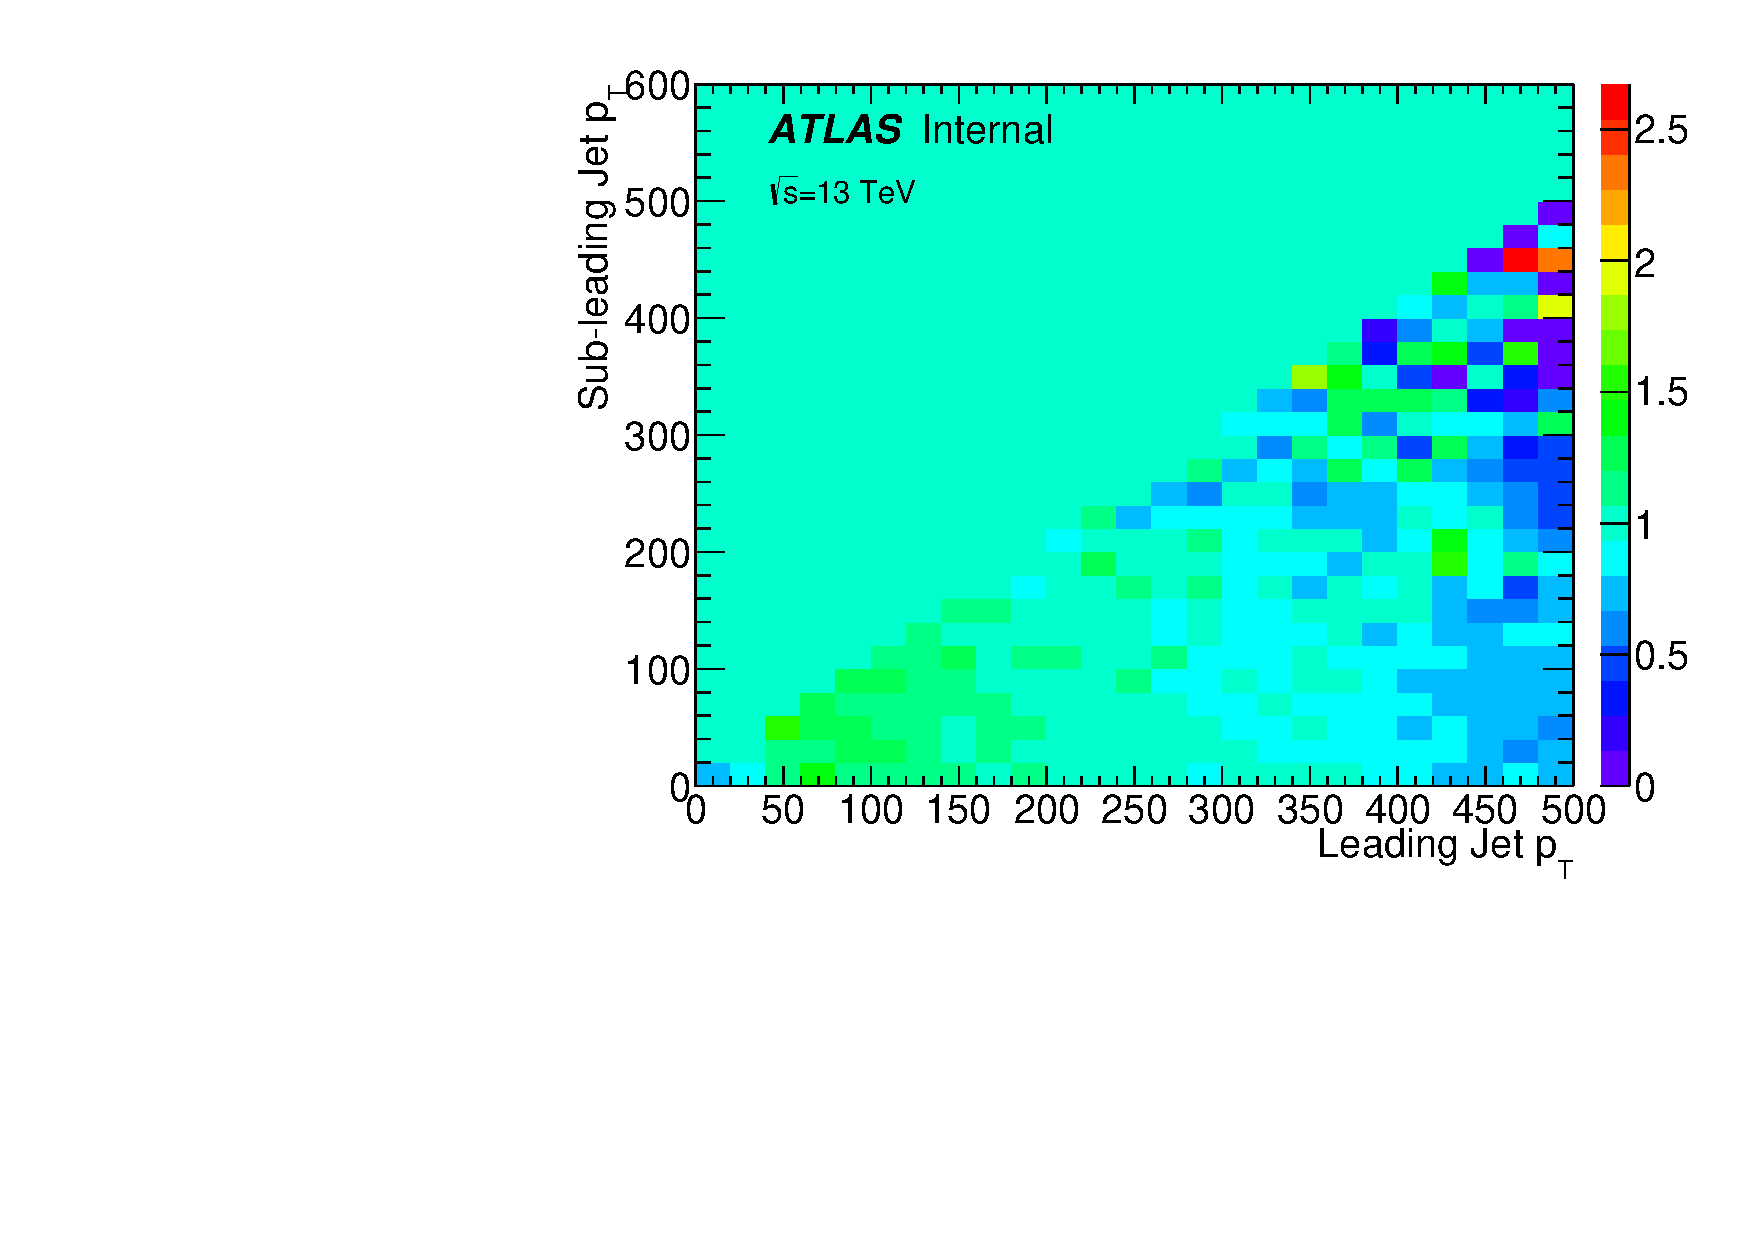
\includegraphics[width=0.6\textwidth]{figures/gbb/pTReweightMap.pdf}
\caption{The re-weighting factor applied to MC as a function of leading and sub-leading track jet $p_T$.}
  \label{fig:gbb-reweightmap}
\end{figure}


\begin{figure}[htbp]
  \centering
 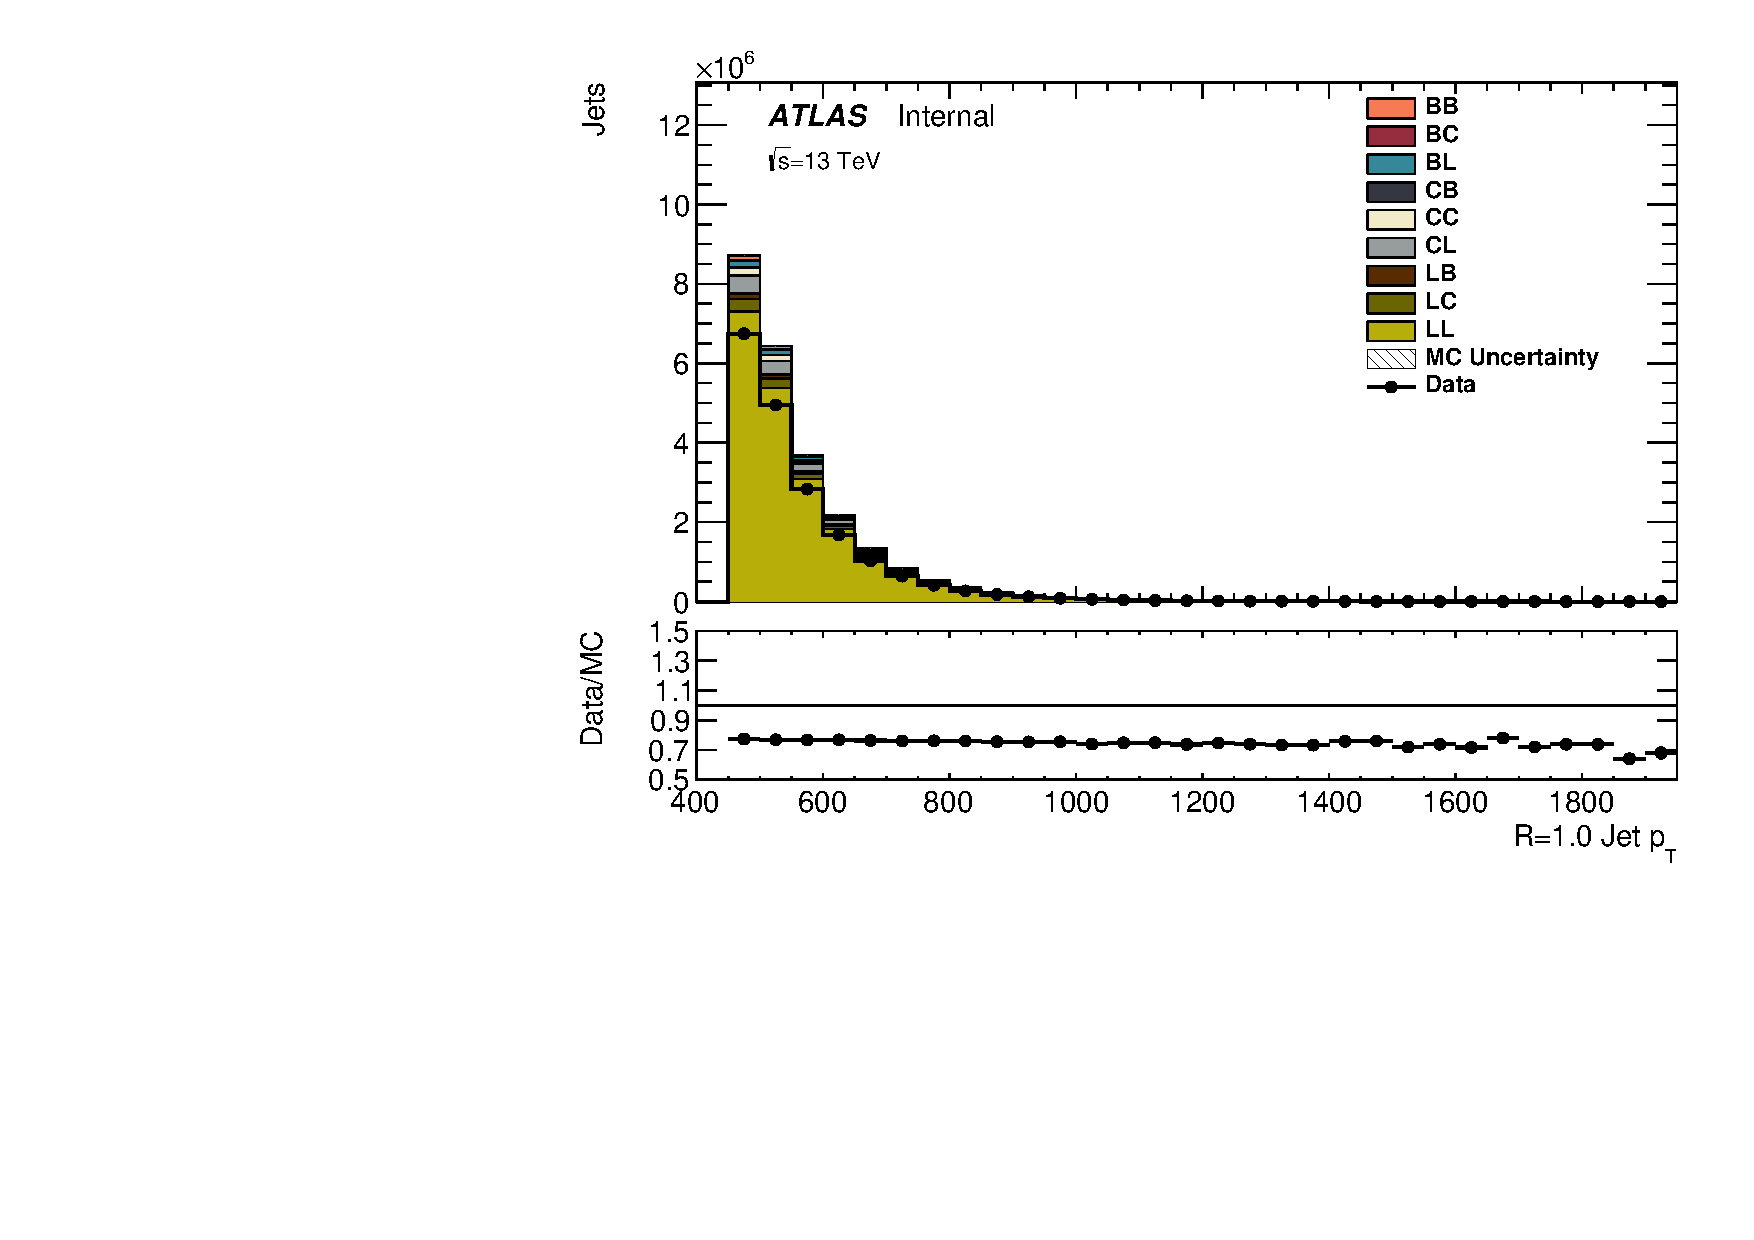
\includegraphics[width=0.45\textwidth]{figures/gbb/LargeRJet_pT_NoReweight.pdf}
 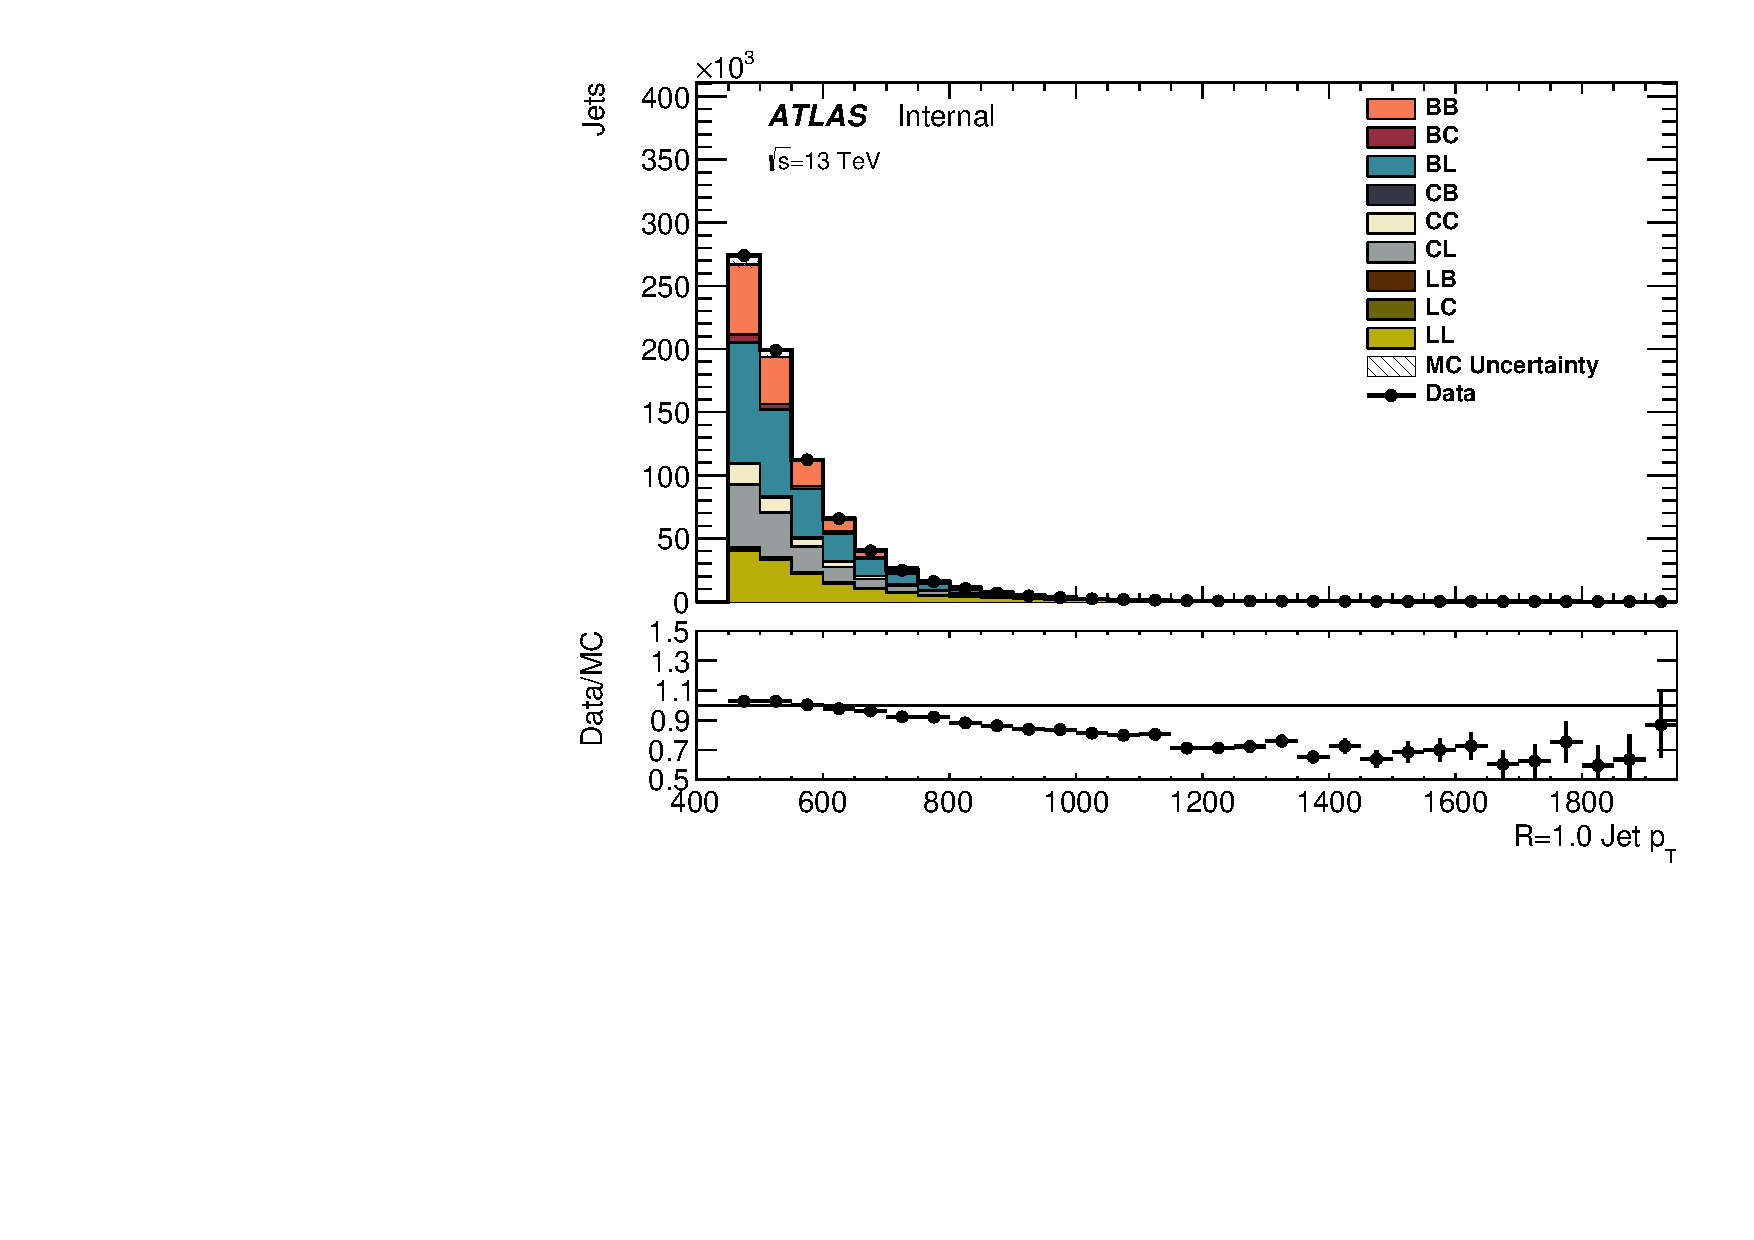
\includegraphics[width=0.45\textwidth]{figures/gbb/LargeRJet_pT_PreReweight.pdf}\\ 
 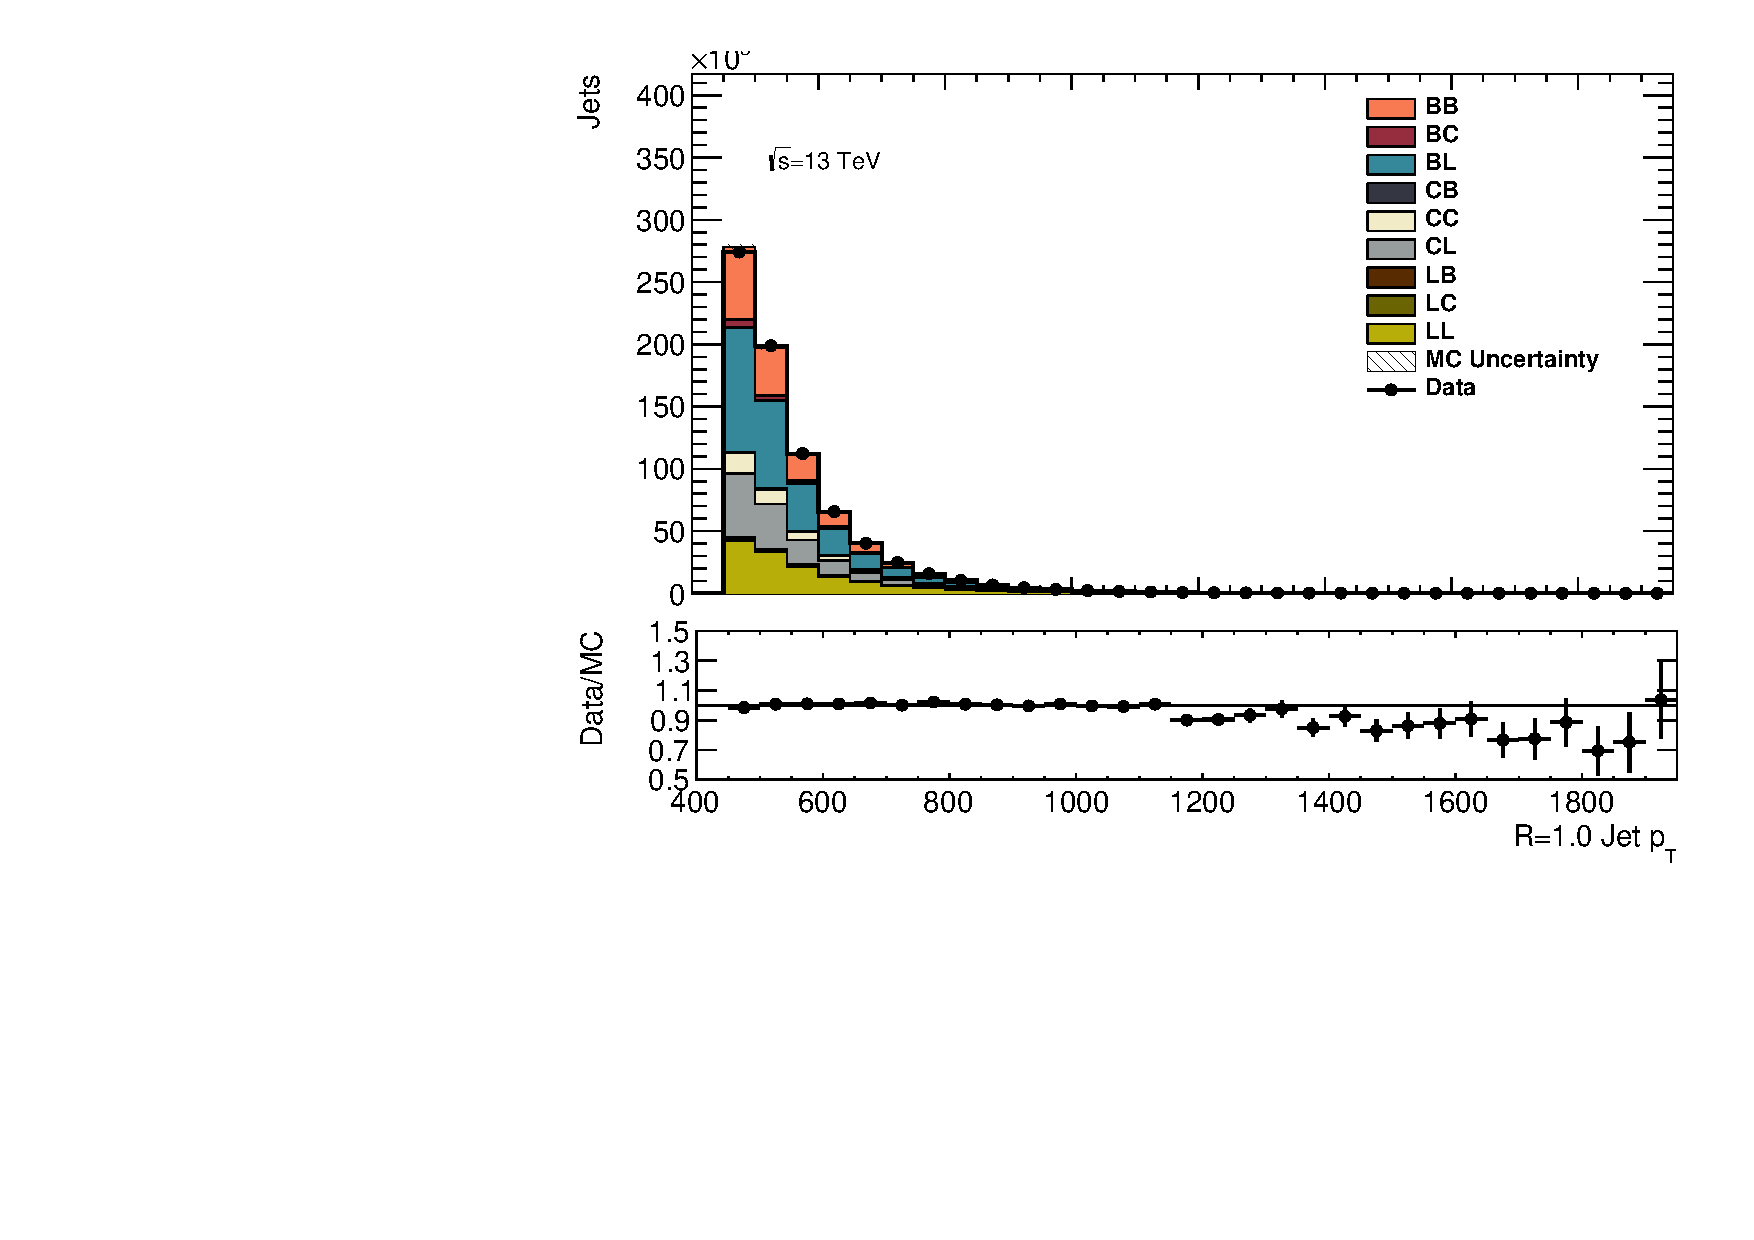
\includegraphics[width=0.45\textwidth]{figures/gbb/LargeRJet_pT_Reweight.pdf}
\caption{Data/MC comparison of $R=1.0$ jet $p_T$ before applying $b$-tagging (top left), post $b$-tagging without kinematic reweighting (top right) and post $b$-tagging with kinematic reweighting (bottom). The label of the $R=1.0$ jet flavor content ``XY'' denotes the leading and sub-leading track jet flavor. For example, the flavors of the leading and sub-leading track jet of a ``BL'' $R=1.0$ jet are `B' and `Light' respectively.}
  \label{fig:gbb-pT_largeR}
\end{figure}


\begin{figure}[htbp]
  \centering
 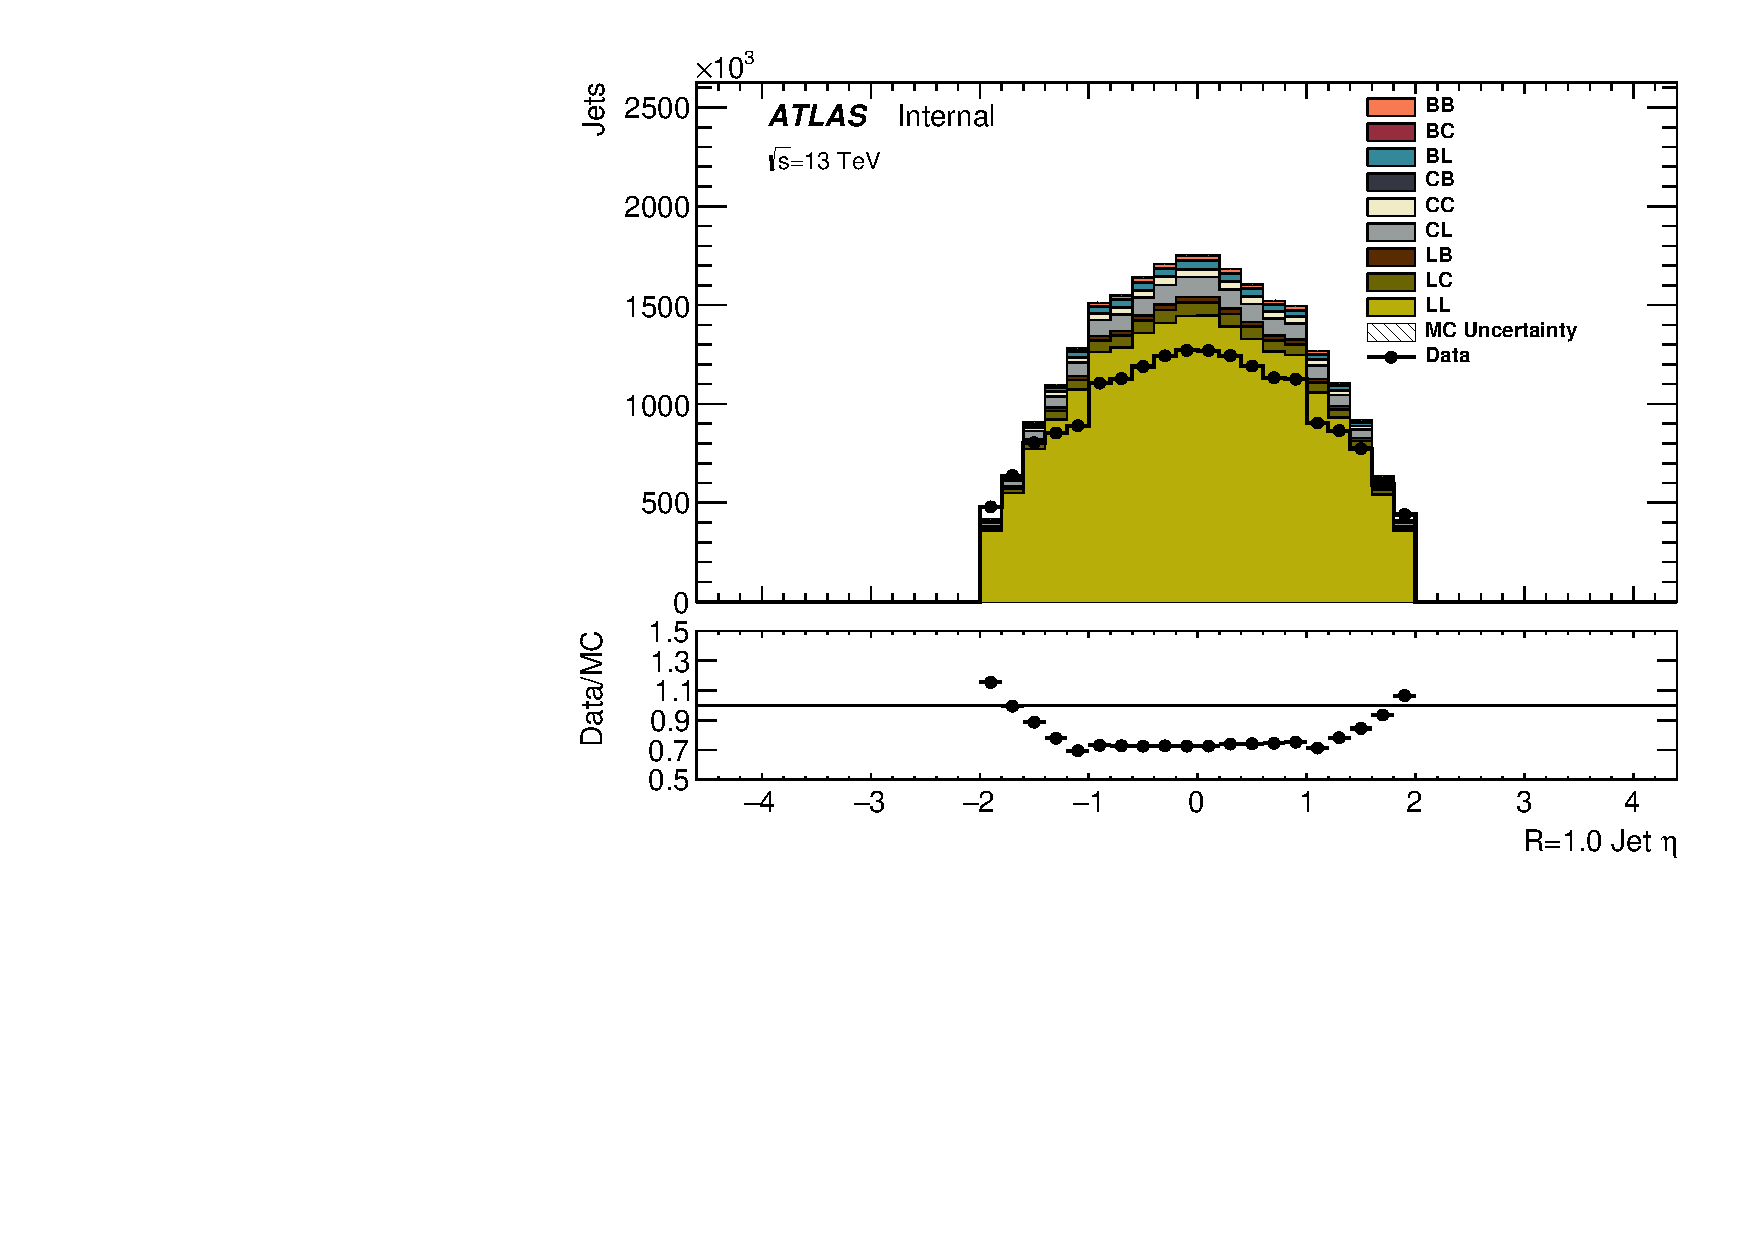
\includegraphics[width=0.45\textwidth]{figures/gbb/LargeRJet_eta_NoReweight.pdf}
 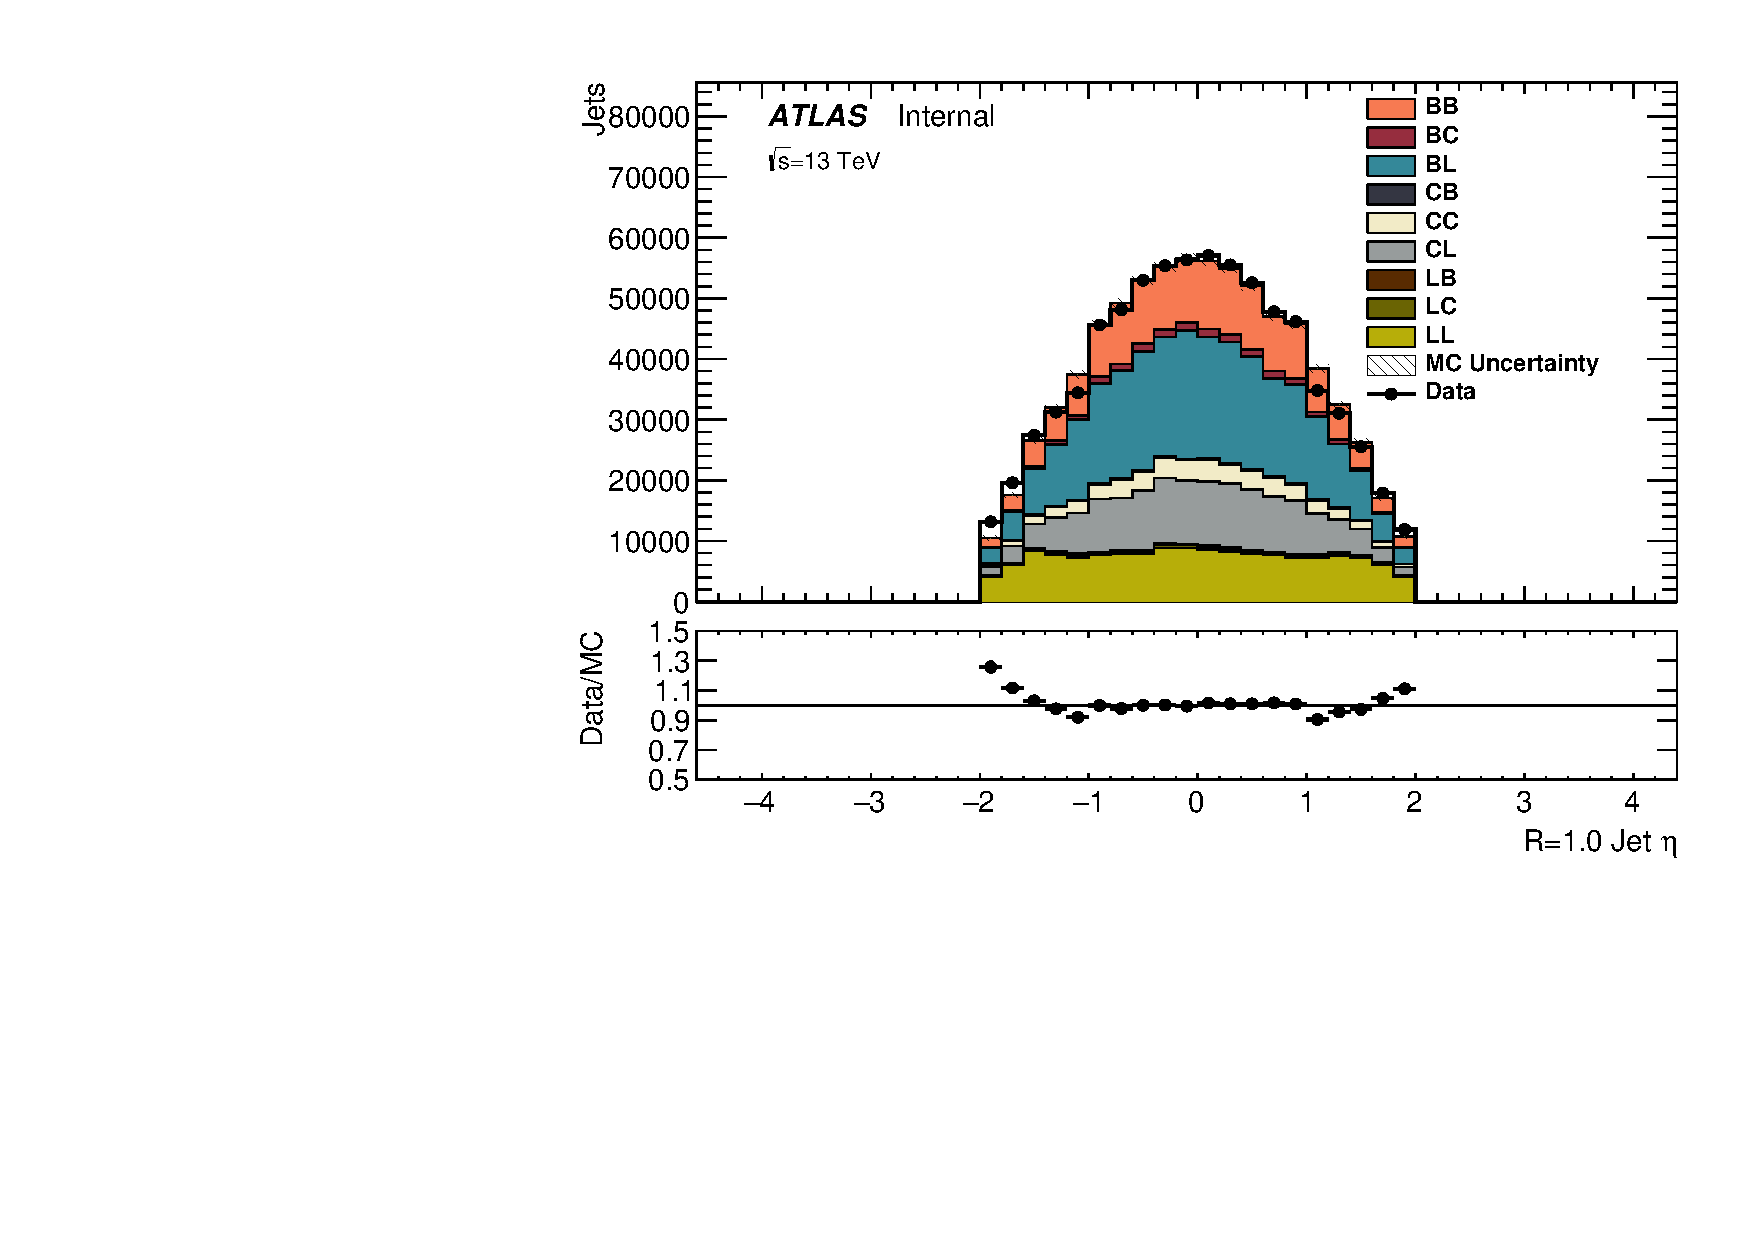
\includegraphics[width=0.45\textwidth]{figures/gbb/LargeRJet_eta_PreReweight.pdf}\\
 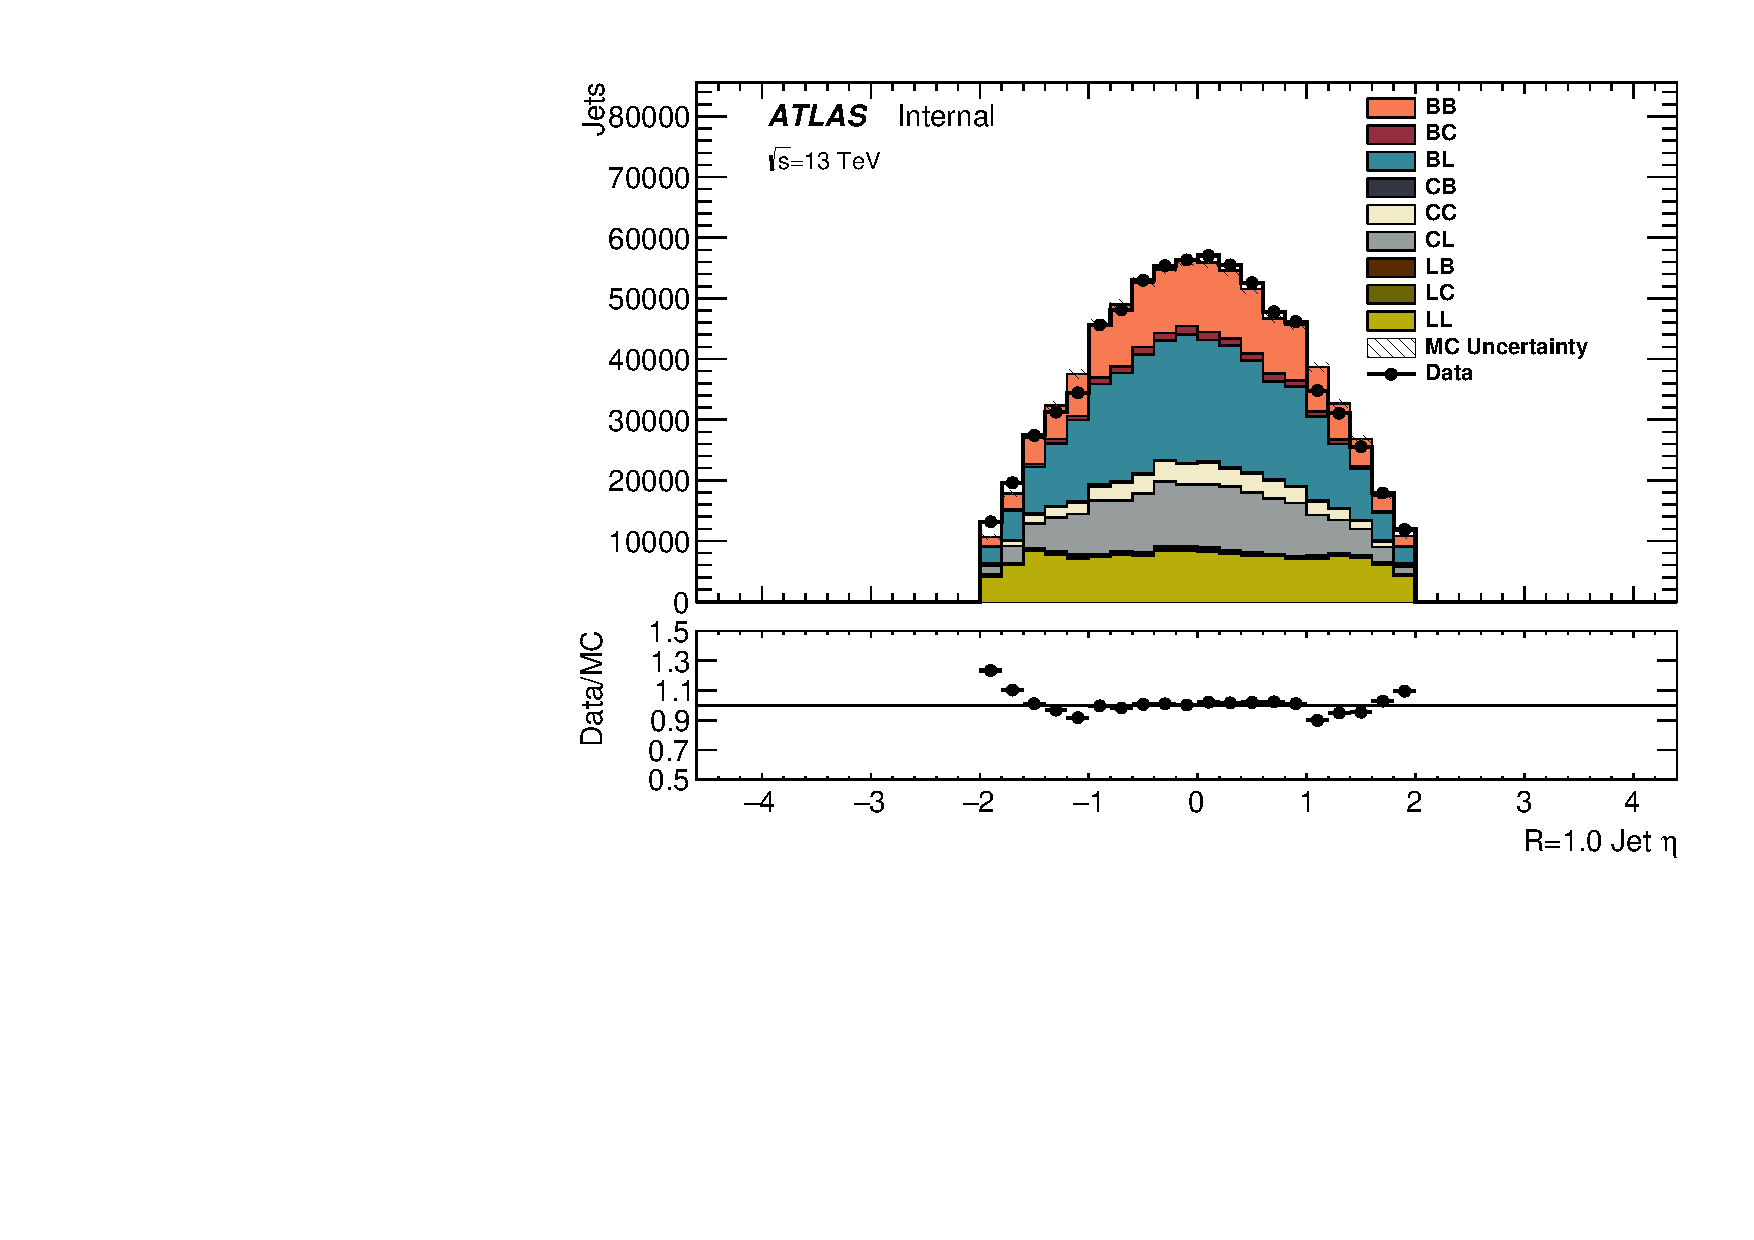
\includegraphics[width=0.45\textwidth]{figures/gbb/LargeRJet_eta_Reweight.pdf}
\caption{Data/MC comparison of $R=1.0$ jet $\eta$ before applying $b$-tagging (top left), post $b$-tagging without kinematic reweighting (top right) and post $b$-tagging with kinematic reweighting (bottom). The label of the $R=1.0$ jet flavor content ``XY'' denotes the leading and sub-leading track jet flavor. For example, the flavors of the leading and sub-leading track jet of a ``BL'' $R=1.0$ jet are `B' and `Light' respectively.}
  \label{fig:gbb-eta_largeR}
\end{figure}



\begin{figure}[htbp]
  \centering
 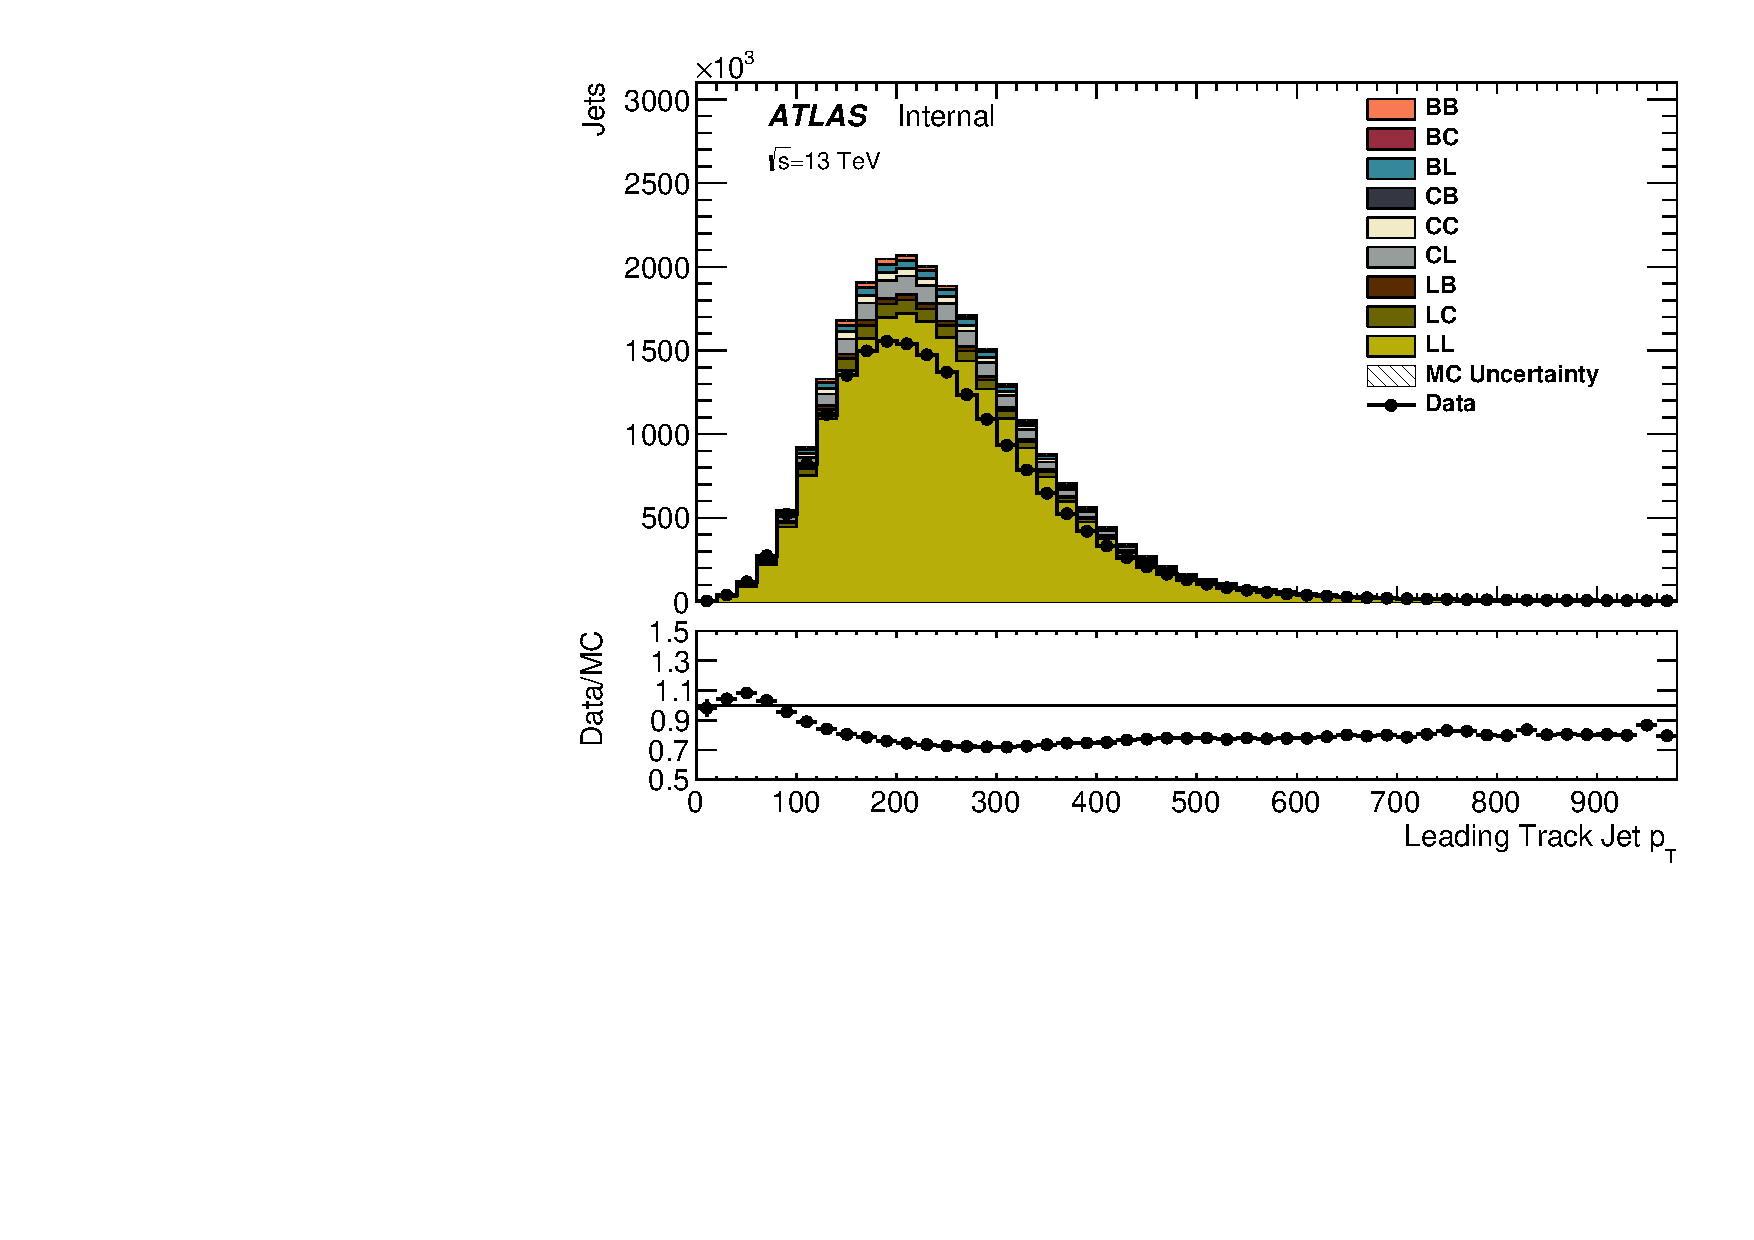
\includegraphics[width=0.45\textwidth]{figures/gbb/LeadTrkJet_pT_NoReweight.pdf}
 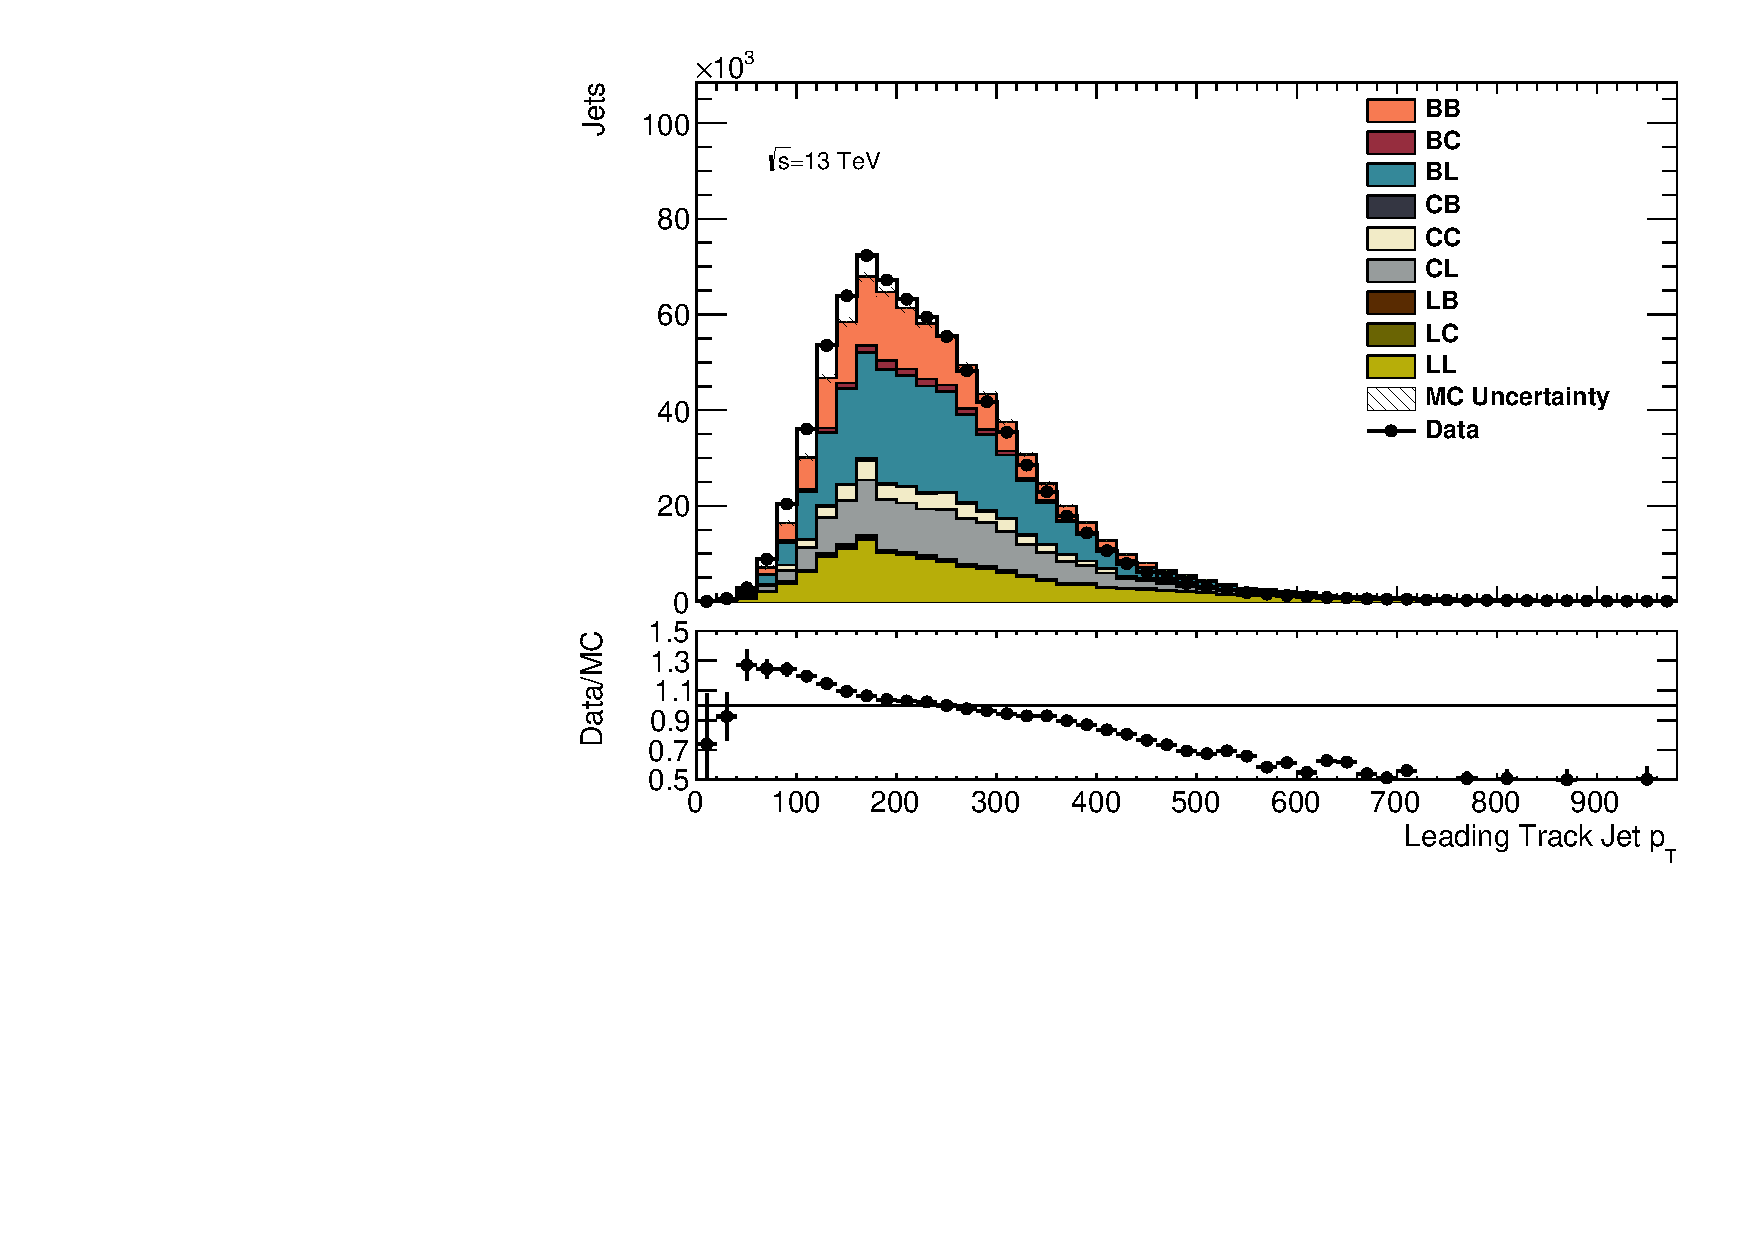
\includegraphics[width=0.45\textwidth]{figures/gbb/LeadTrkJet_pT_PreReweight.pdf}\\
 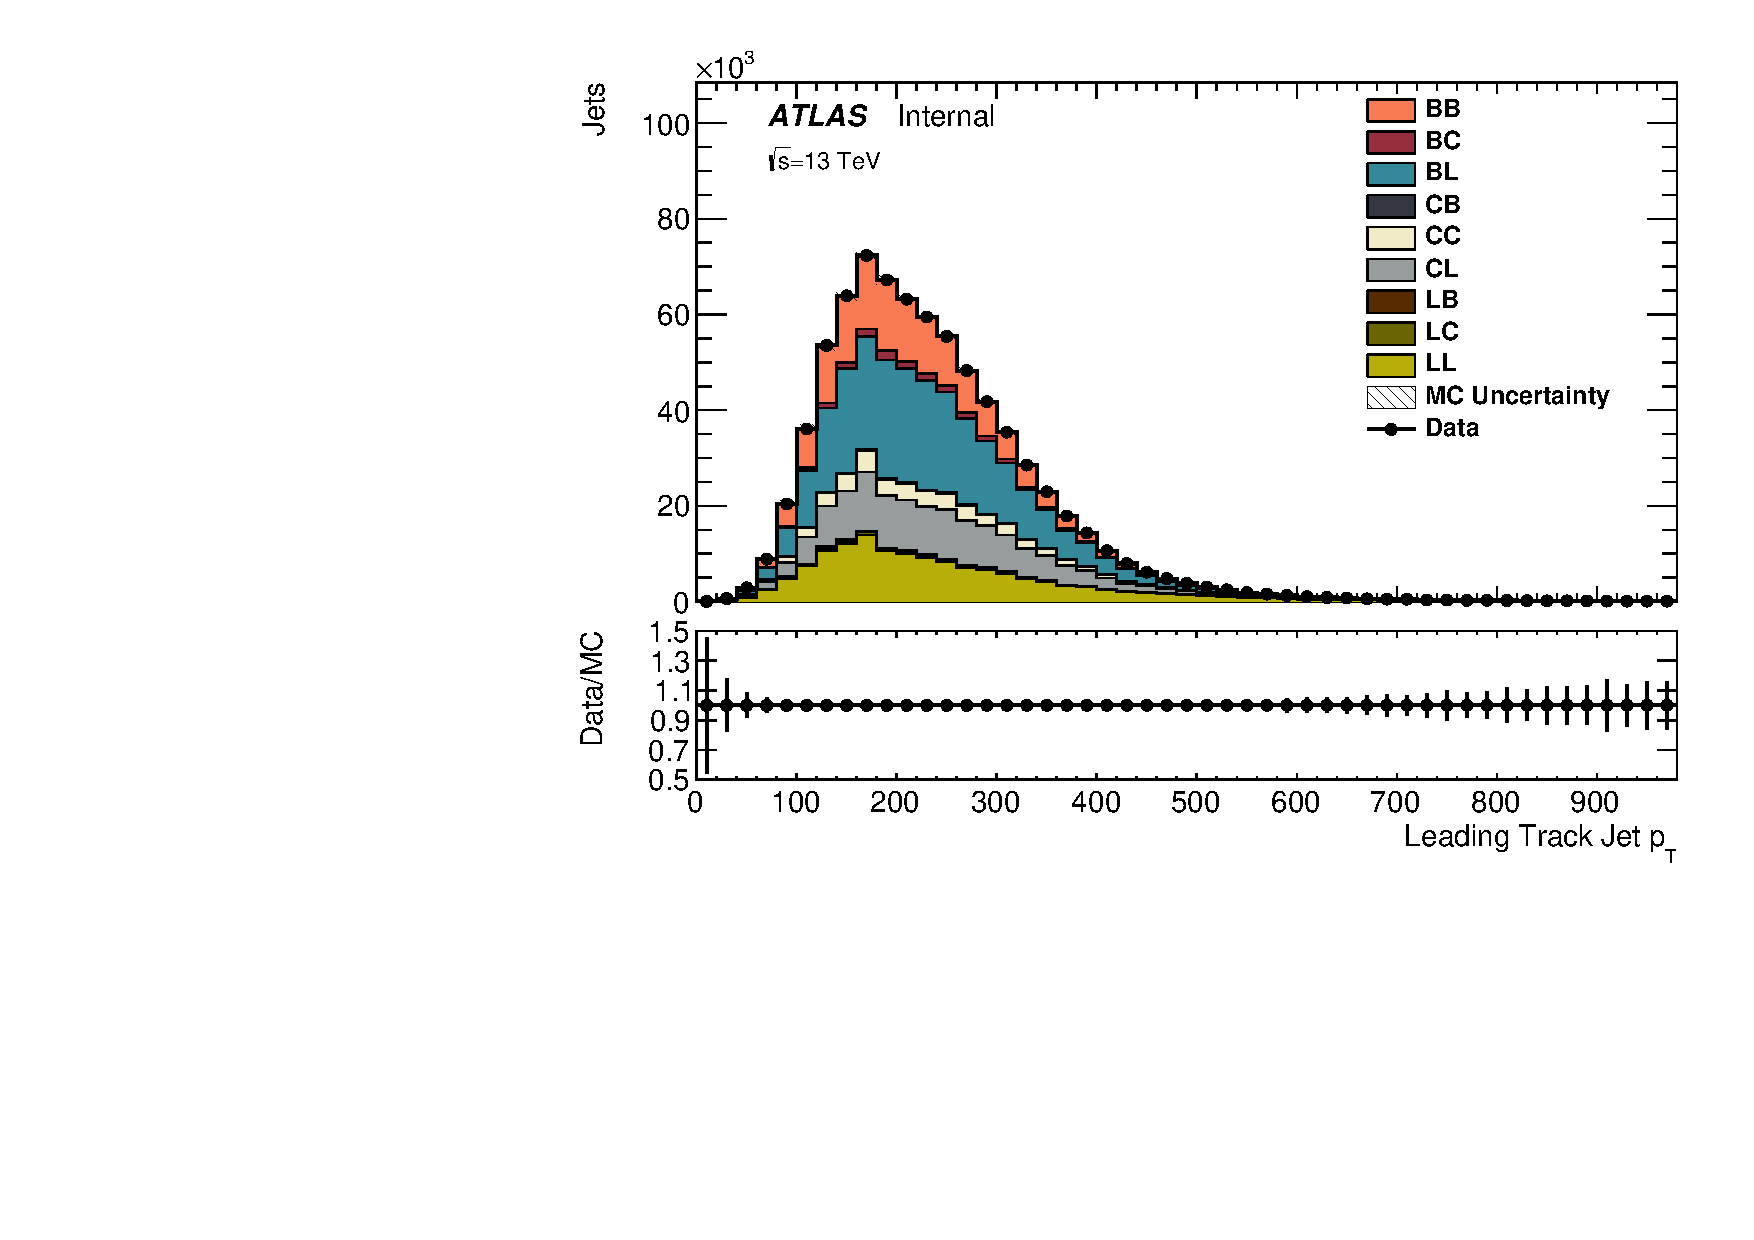
\includegraphics[width=0.45\textwidth]{figures/gbb/LeadTrkJet_pT_Reweight.pdf}
\caption{Data/MC comparison of leading track jets $p_T$ before applying $b$-tagging (top left), post $b$-tagging without kinematic reweighting (top right) and post $b$-tagging with kinematic reweighting (bottom). The label of the $R=1.0$ jet flavor content ``XY'' denotes the leading and sub-leading track jet flavor. For example, the flavors of the leading and sub-leading track jet of a ``BL'' $R=1.0$ jet are `B' and `Light' respectively.}
  \label{fig:gbb-pT_leadtrkjets}
\end{figure}


\begin{figure}[htbp]
  \centering
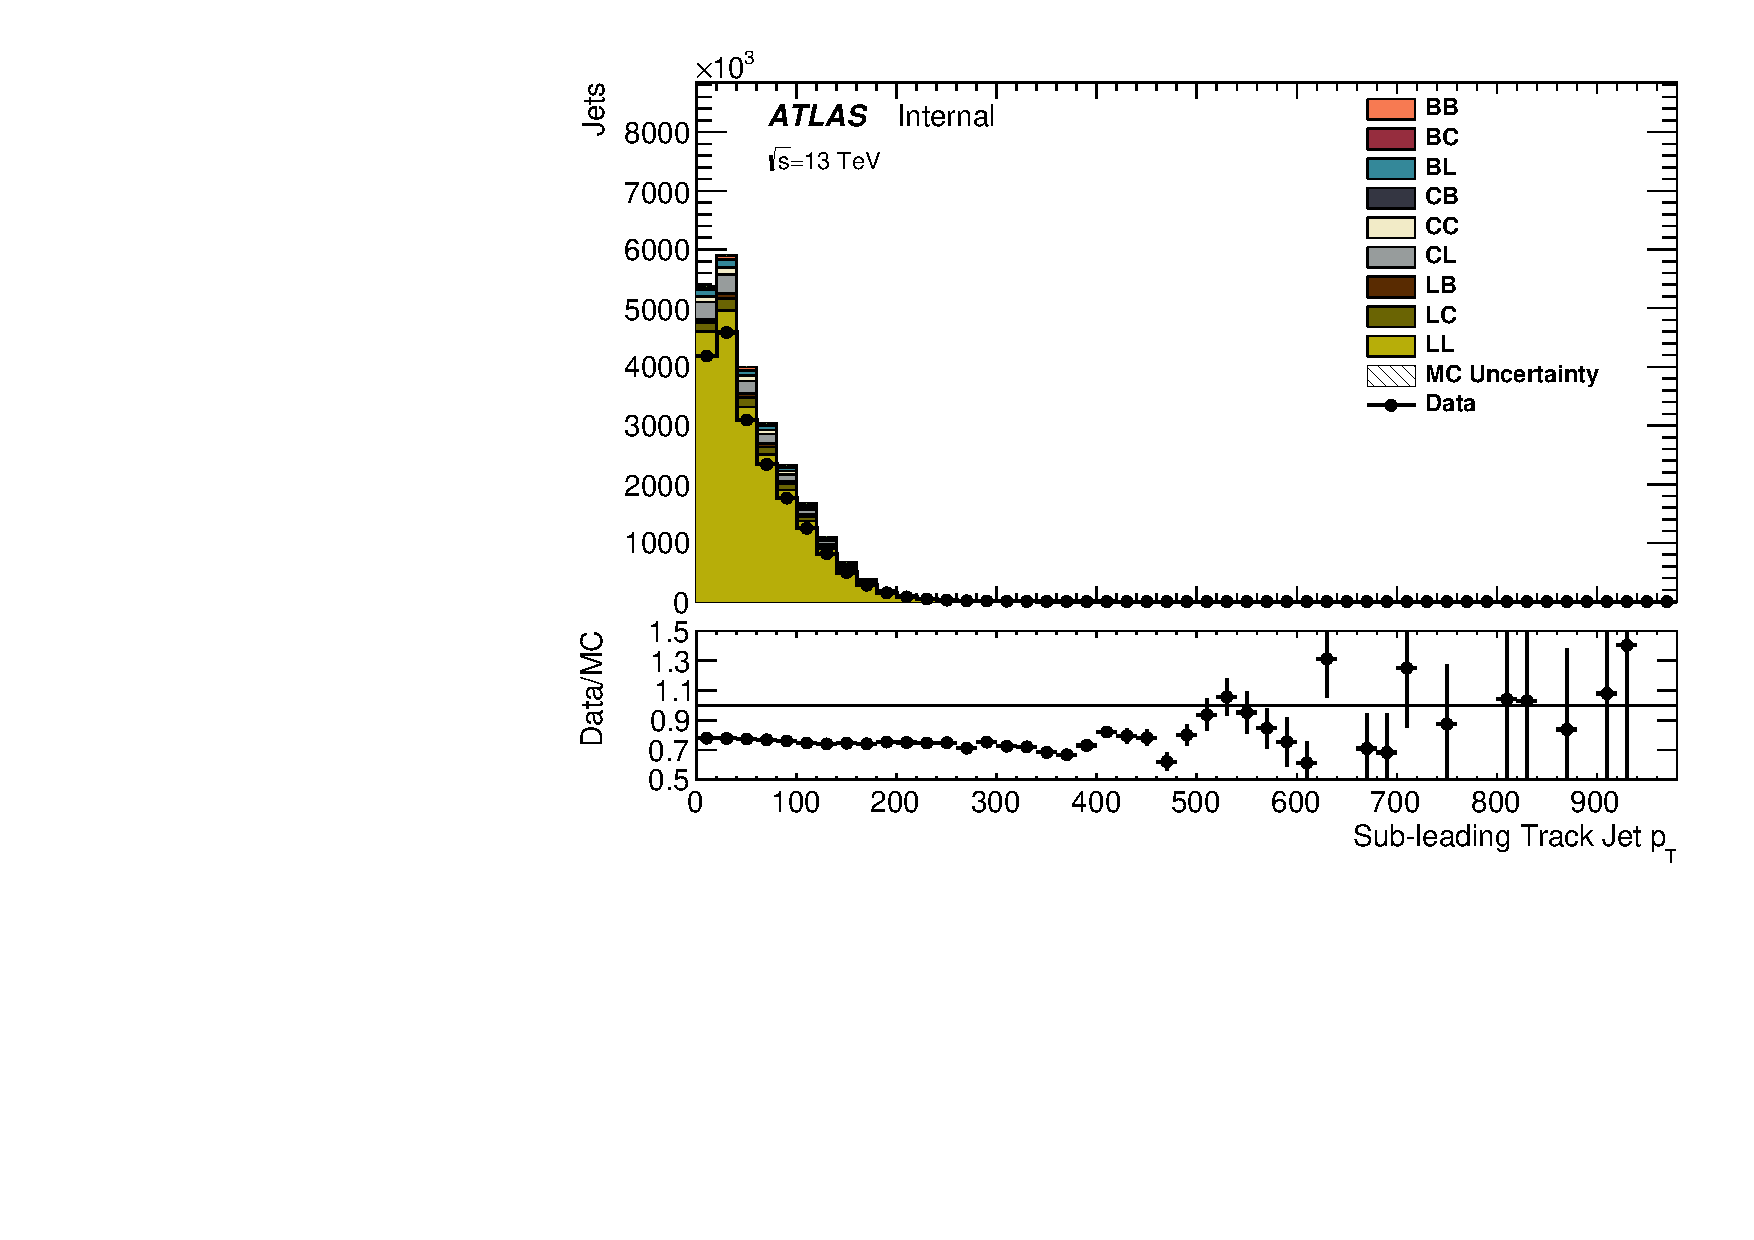
\includegraphics[width=0.45\textwidth]{figures/gbb/SubLeadTrkJet_pT_NoReweight.pdf}
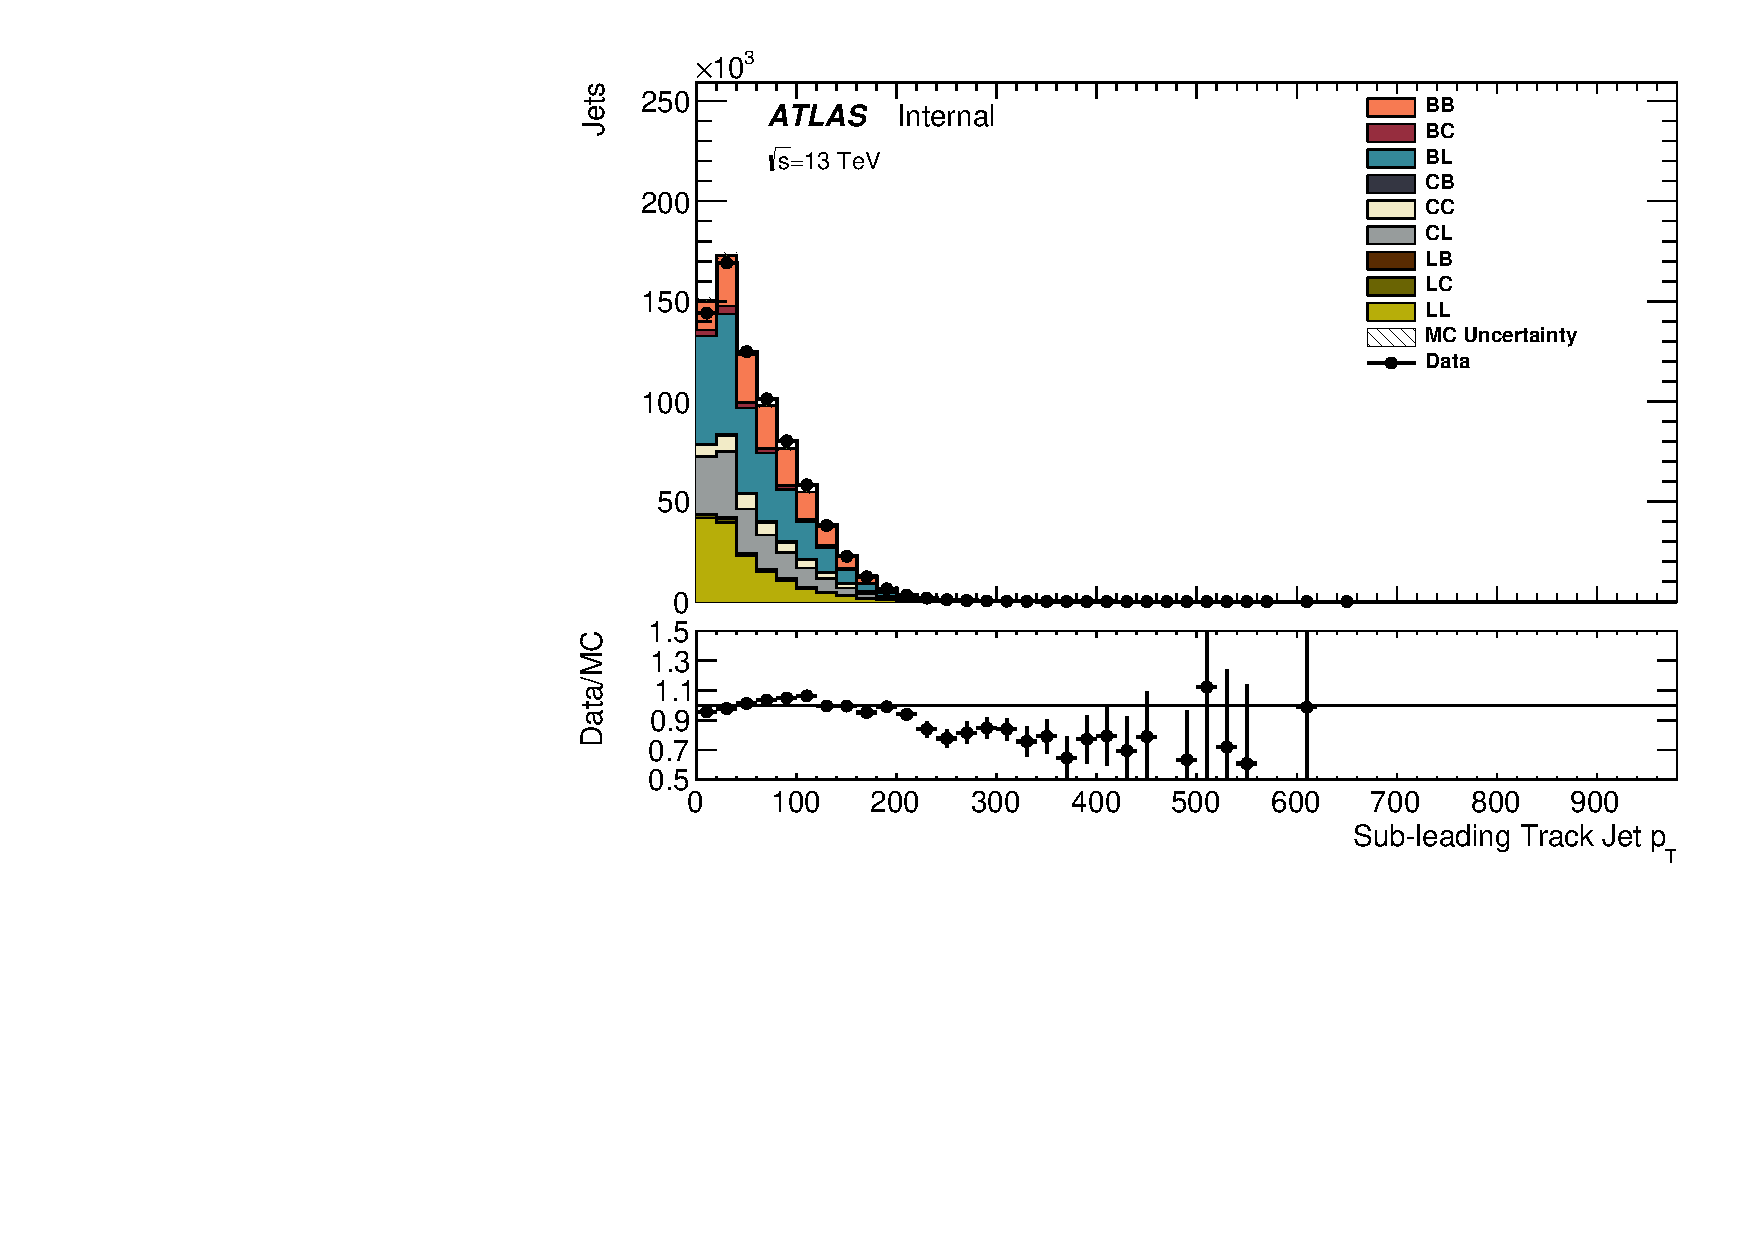
\includegraphics[width=0.45\textwidth]{figures/gbb/SubLeadTrkJet_pT_PreReweight.pdf}\\
 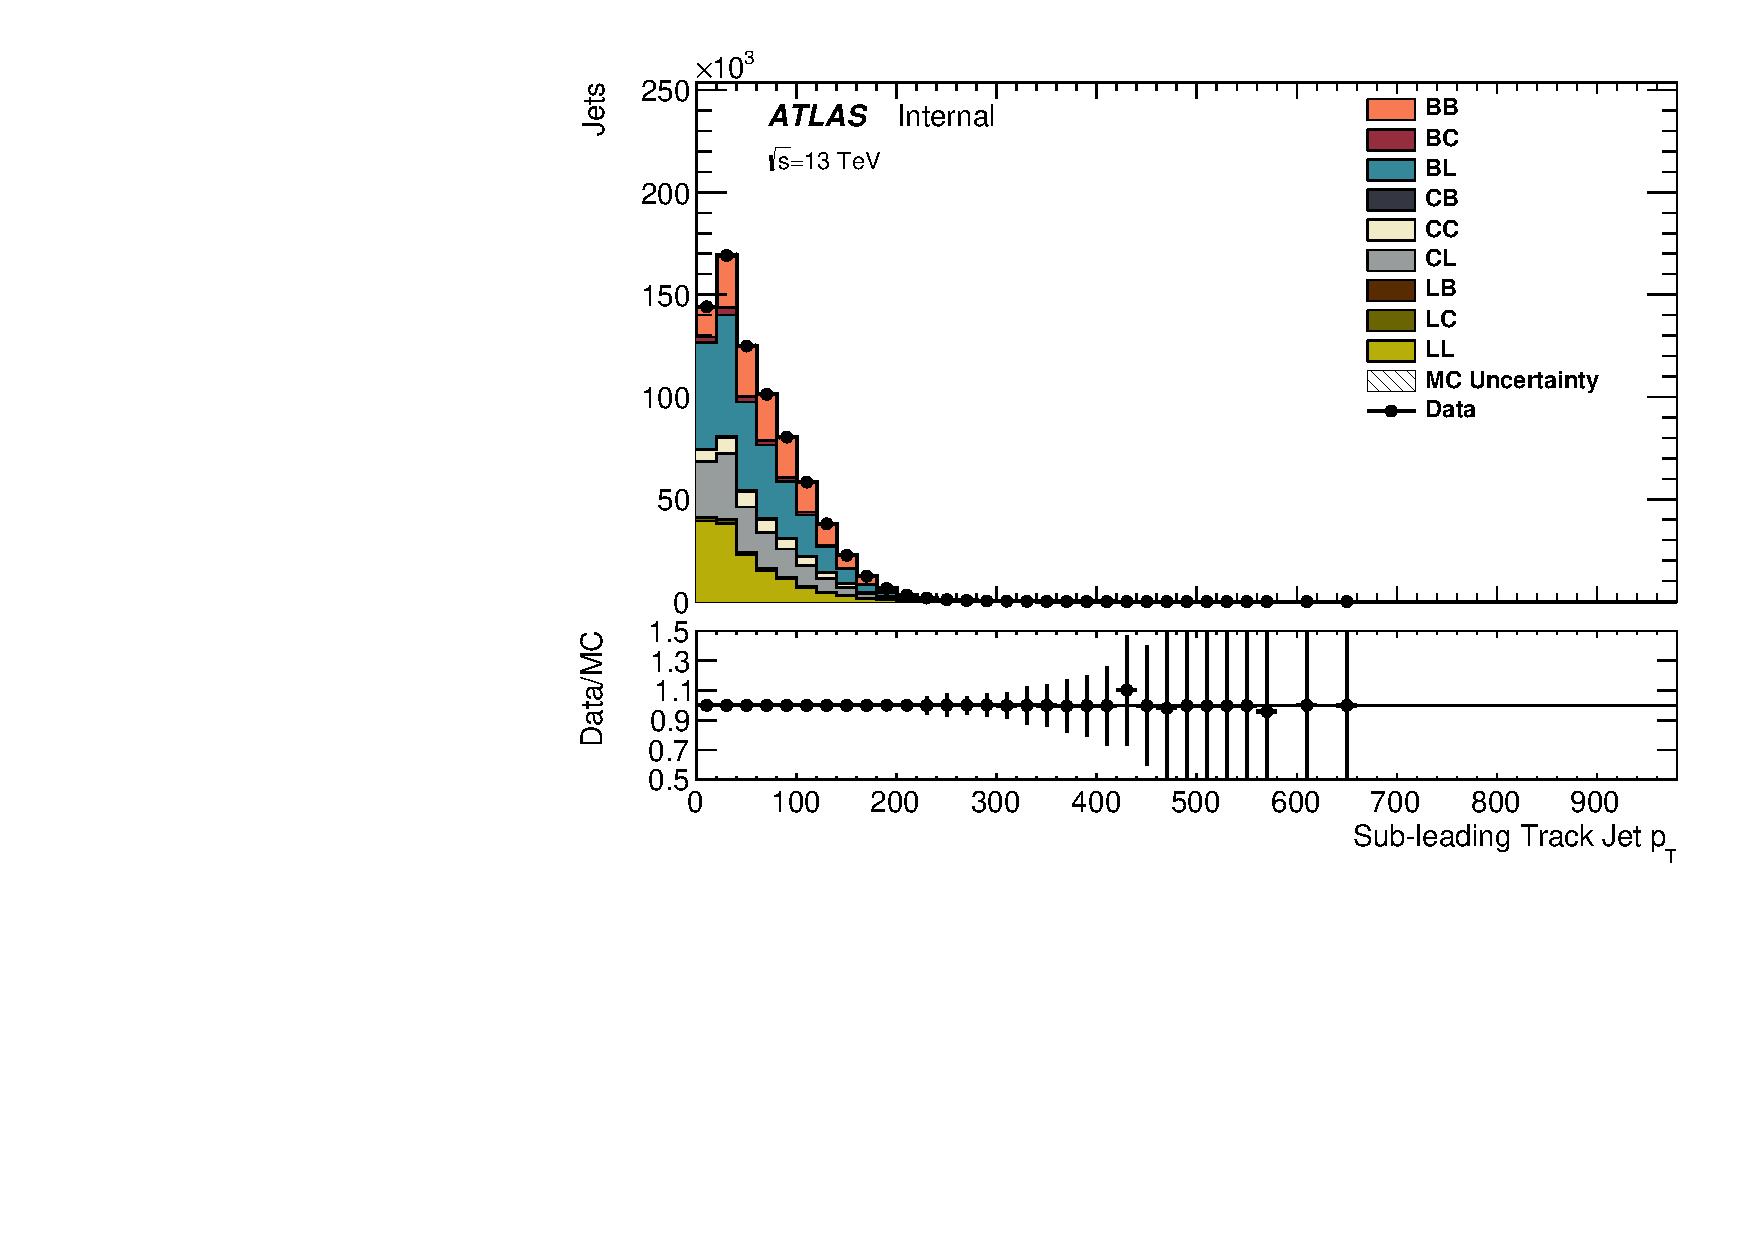
\includegraphics[width=0.45\textwidth]{figures/gbb/SubLeadTrkJet_pT_Reweight.pdf}
\caption{Data/MC comparison of sub-leading track jets $p_T$ before applying $b$-tagging (top left), post $b$-tagging without kinematic reweighting (top right) and post $b$-tagging with kinematic reweighting (bottom). The label of the $R=1.0$ jet flavor content ``XY'' denotes the leading and sub-leading track jet flavor. For example, the flavors of the leading and sub-leading track jet of a ``BL'' $R=1.0$ jet are `B' and `Light' respectively.}
  \label{fig:gbb-pT_subtrkjets}
\end{figure}


\begin{figure}[htbp]
  \centering
 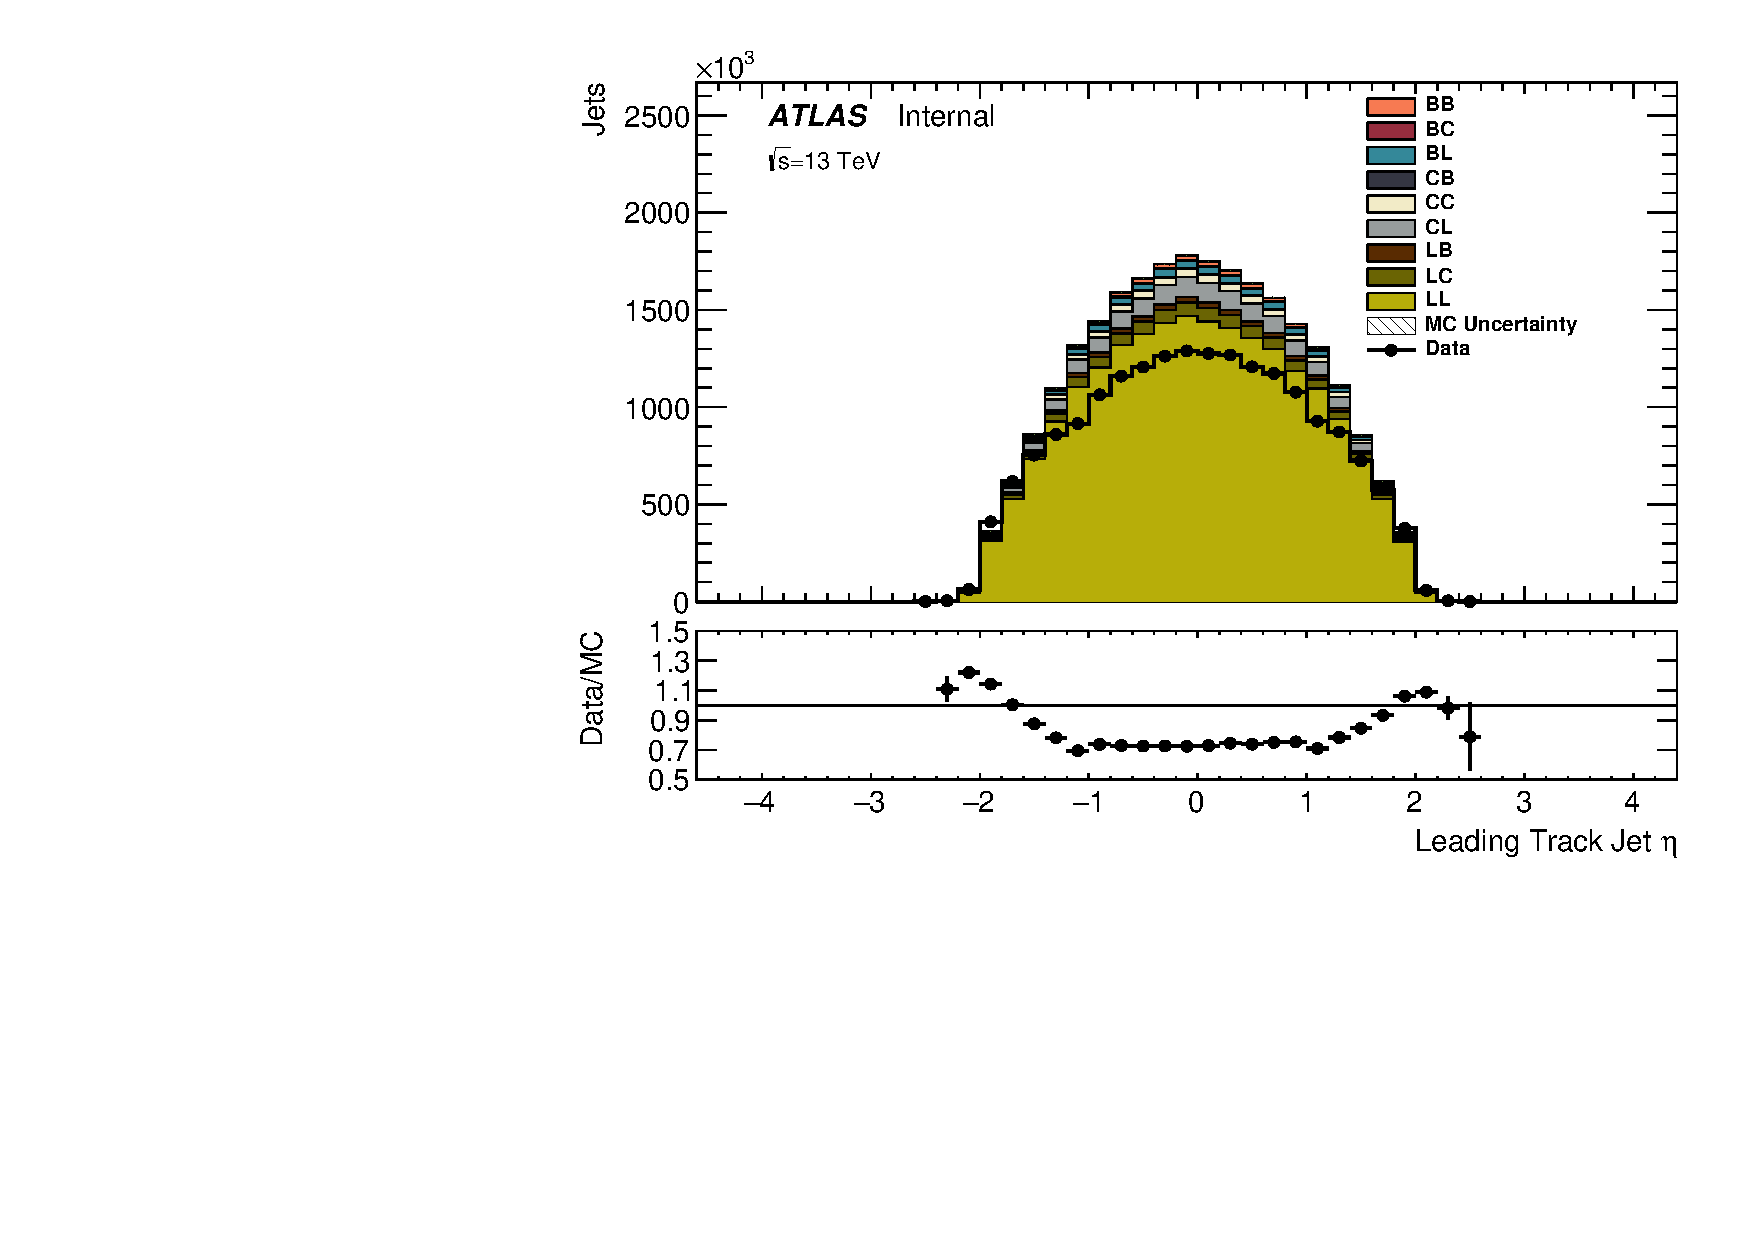
\includegraphics[width=0.45\textwidth]{figures/gbb/LeadTrkJet_eta_NoReweight.pdf}
 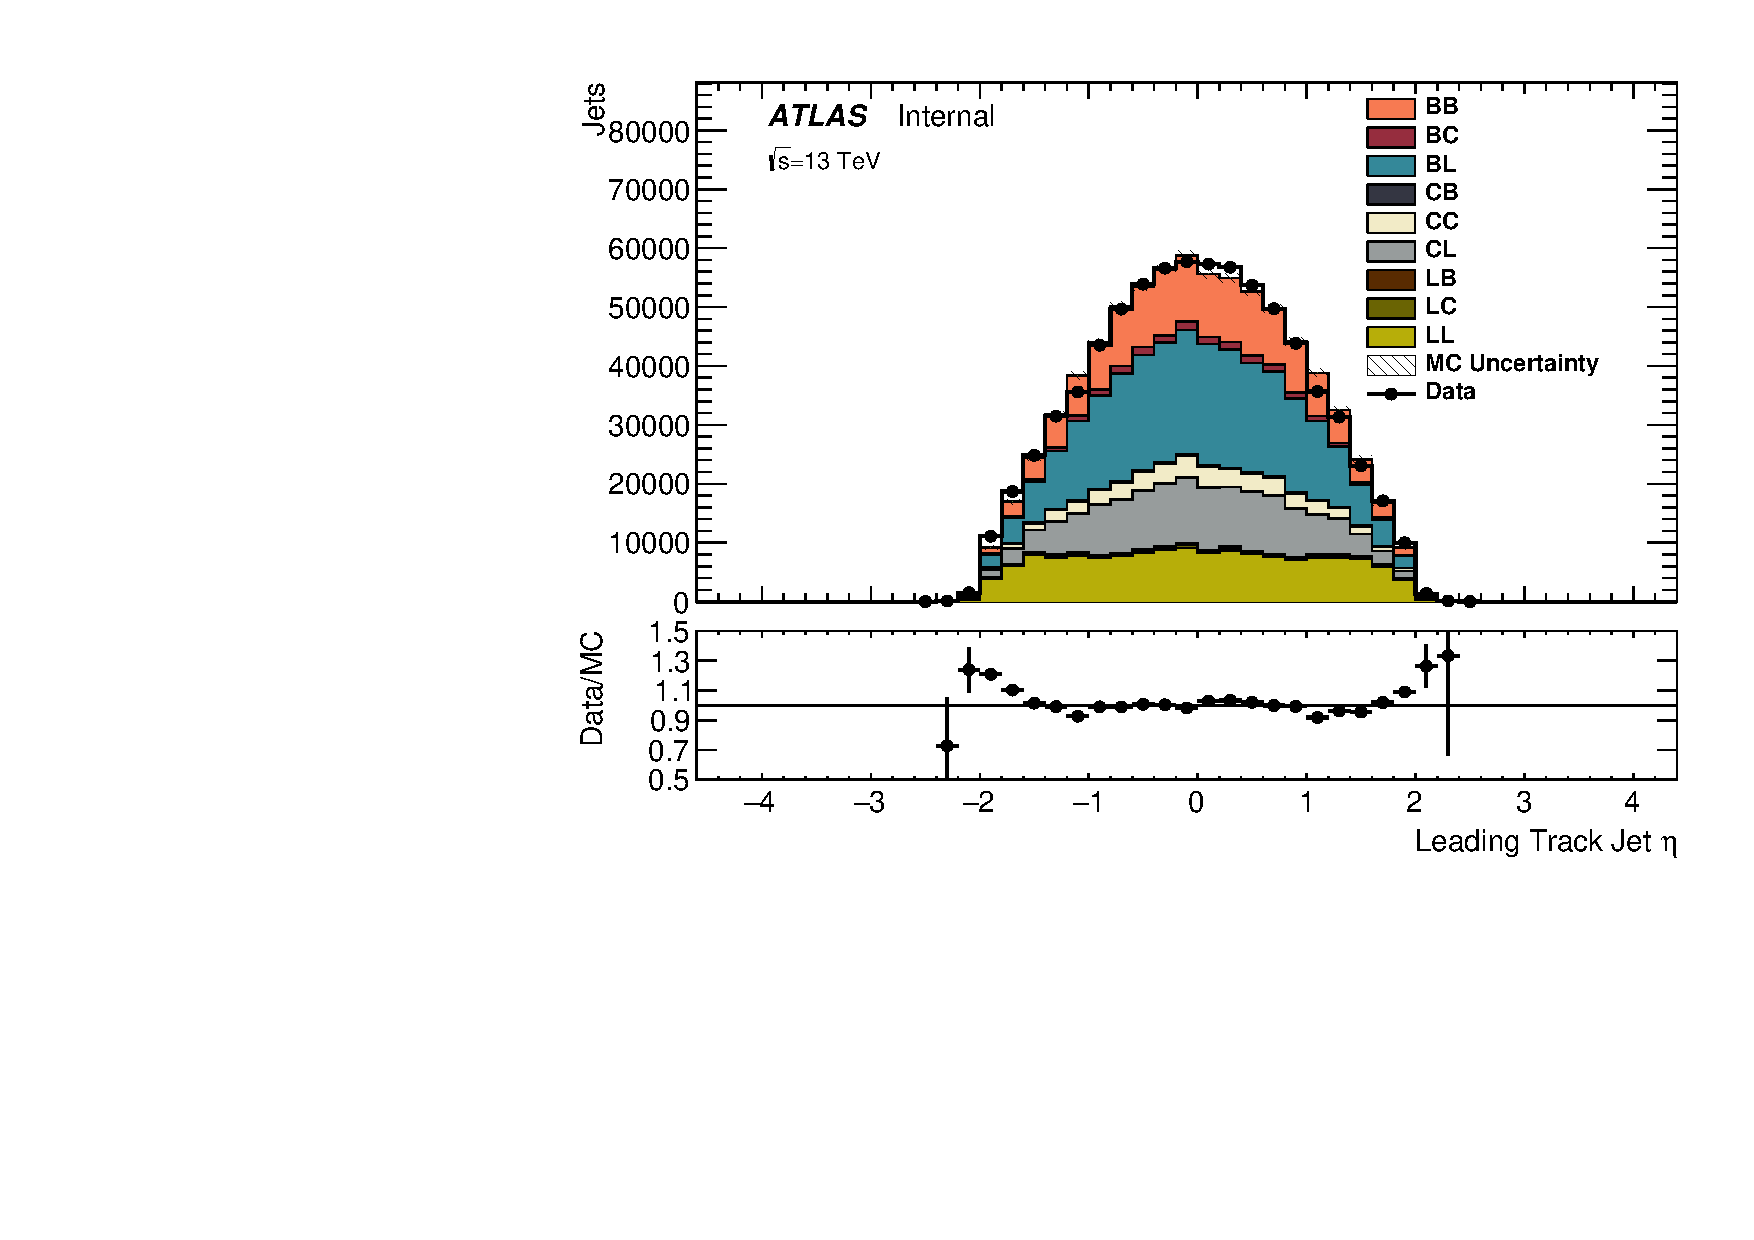
\includegraphics[width=0.45\textwidth]{figures/gbb/LeadTrkJet_eta_PreReweight.pdf}\\
 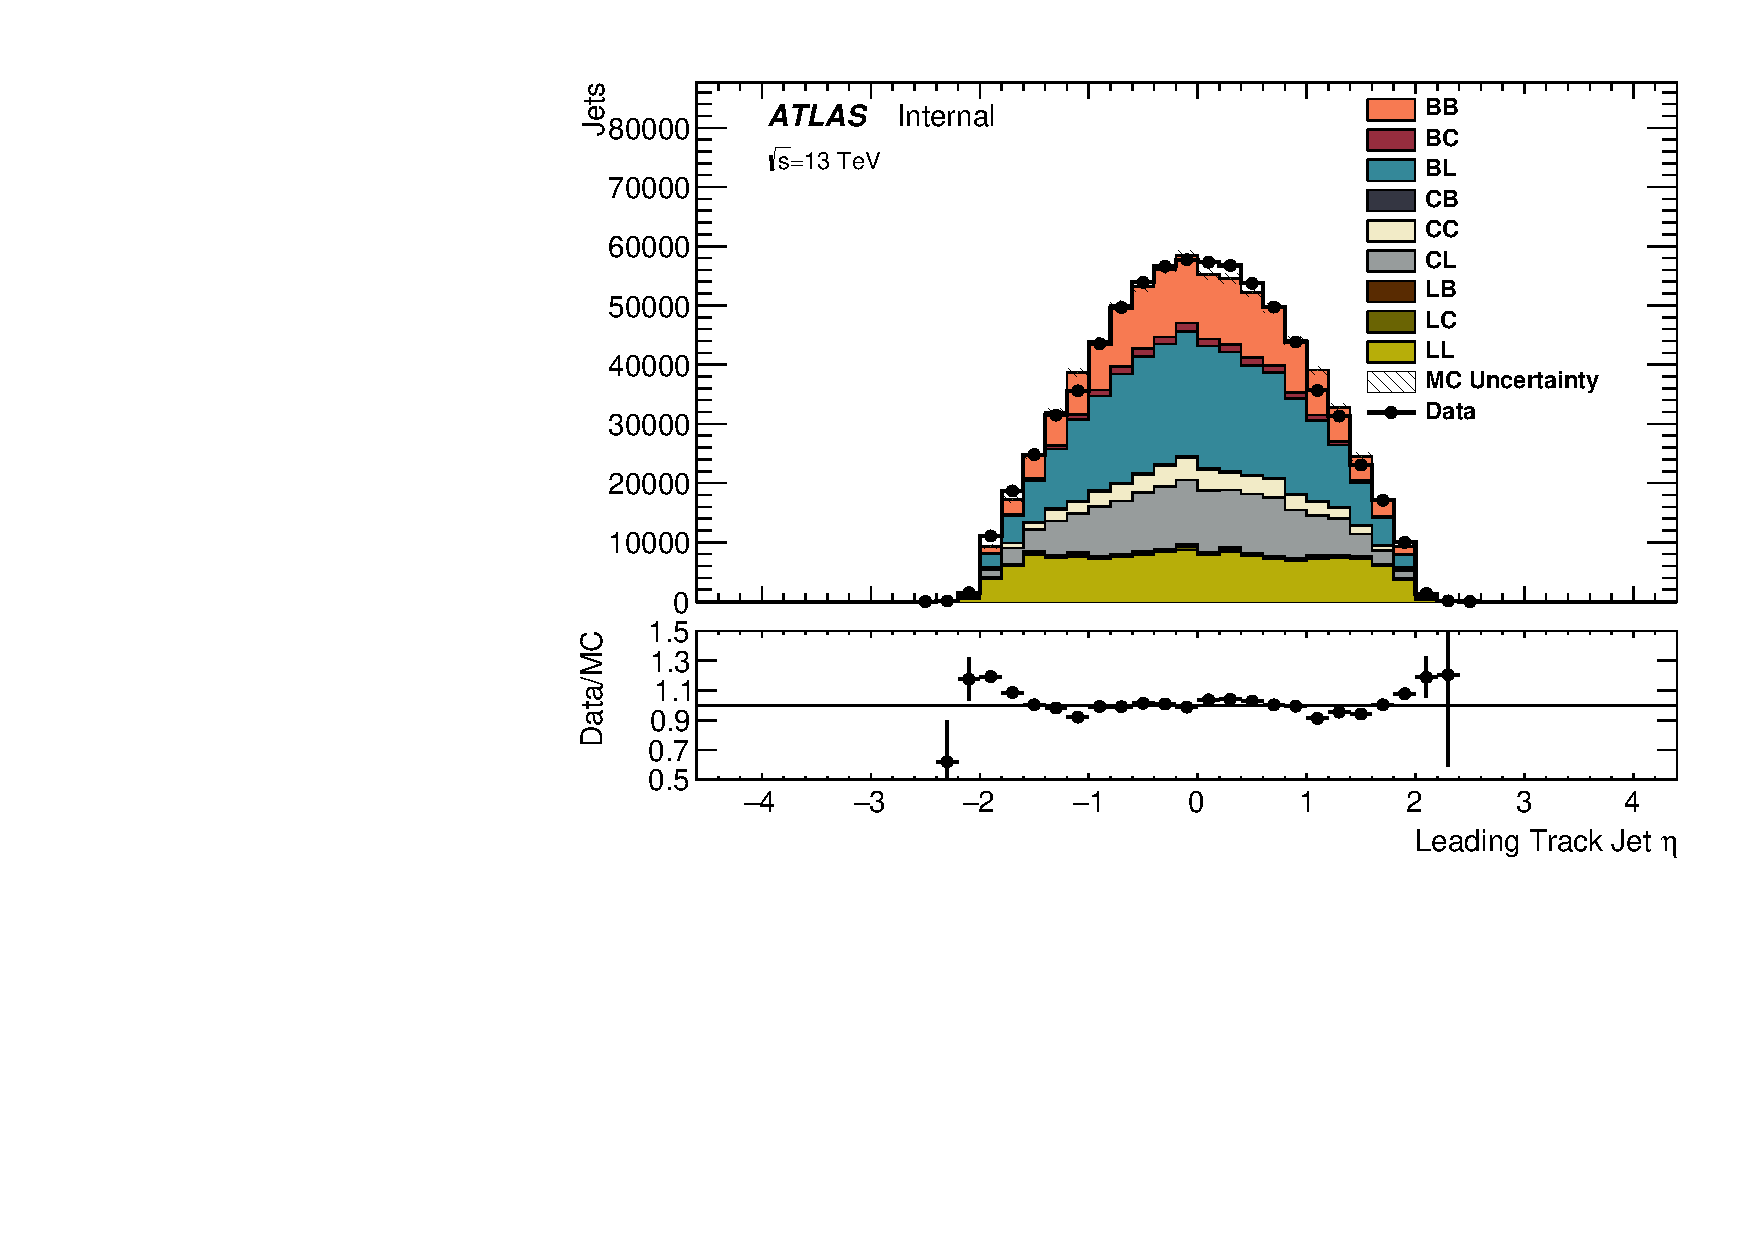
\includegraphics[width=0.45\textwidth]{figures/gbb/LeadTrkJet_eta_Reweight.pdf}
\caption{Data/MC comparison of leading track jets $\eta$ before applying $b$-tagging (top left), post $b$-tagging without kinematic reweighting (top right) and post $b$-tagging with kinematic reweighting (bottom). The label of the $R=1.0$ jet flavor content ``XY'' denotes the leading and sub-leading track jet flavor. For example, the flavors of the leading and sub-leading track jet of a ``BL'' $R=1.0$ jet are `B' and `Light' respectively.}
  \label{fig:gbb-eta_leadtrkjets}
\end{figure}


\begin{figure}[htbp]
  \centering
 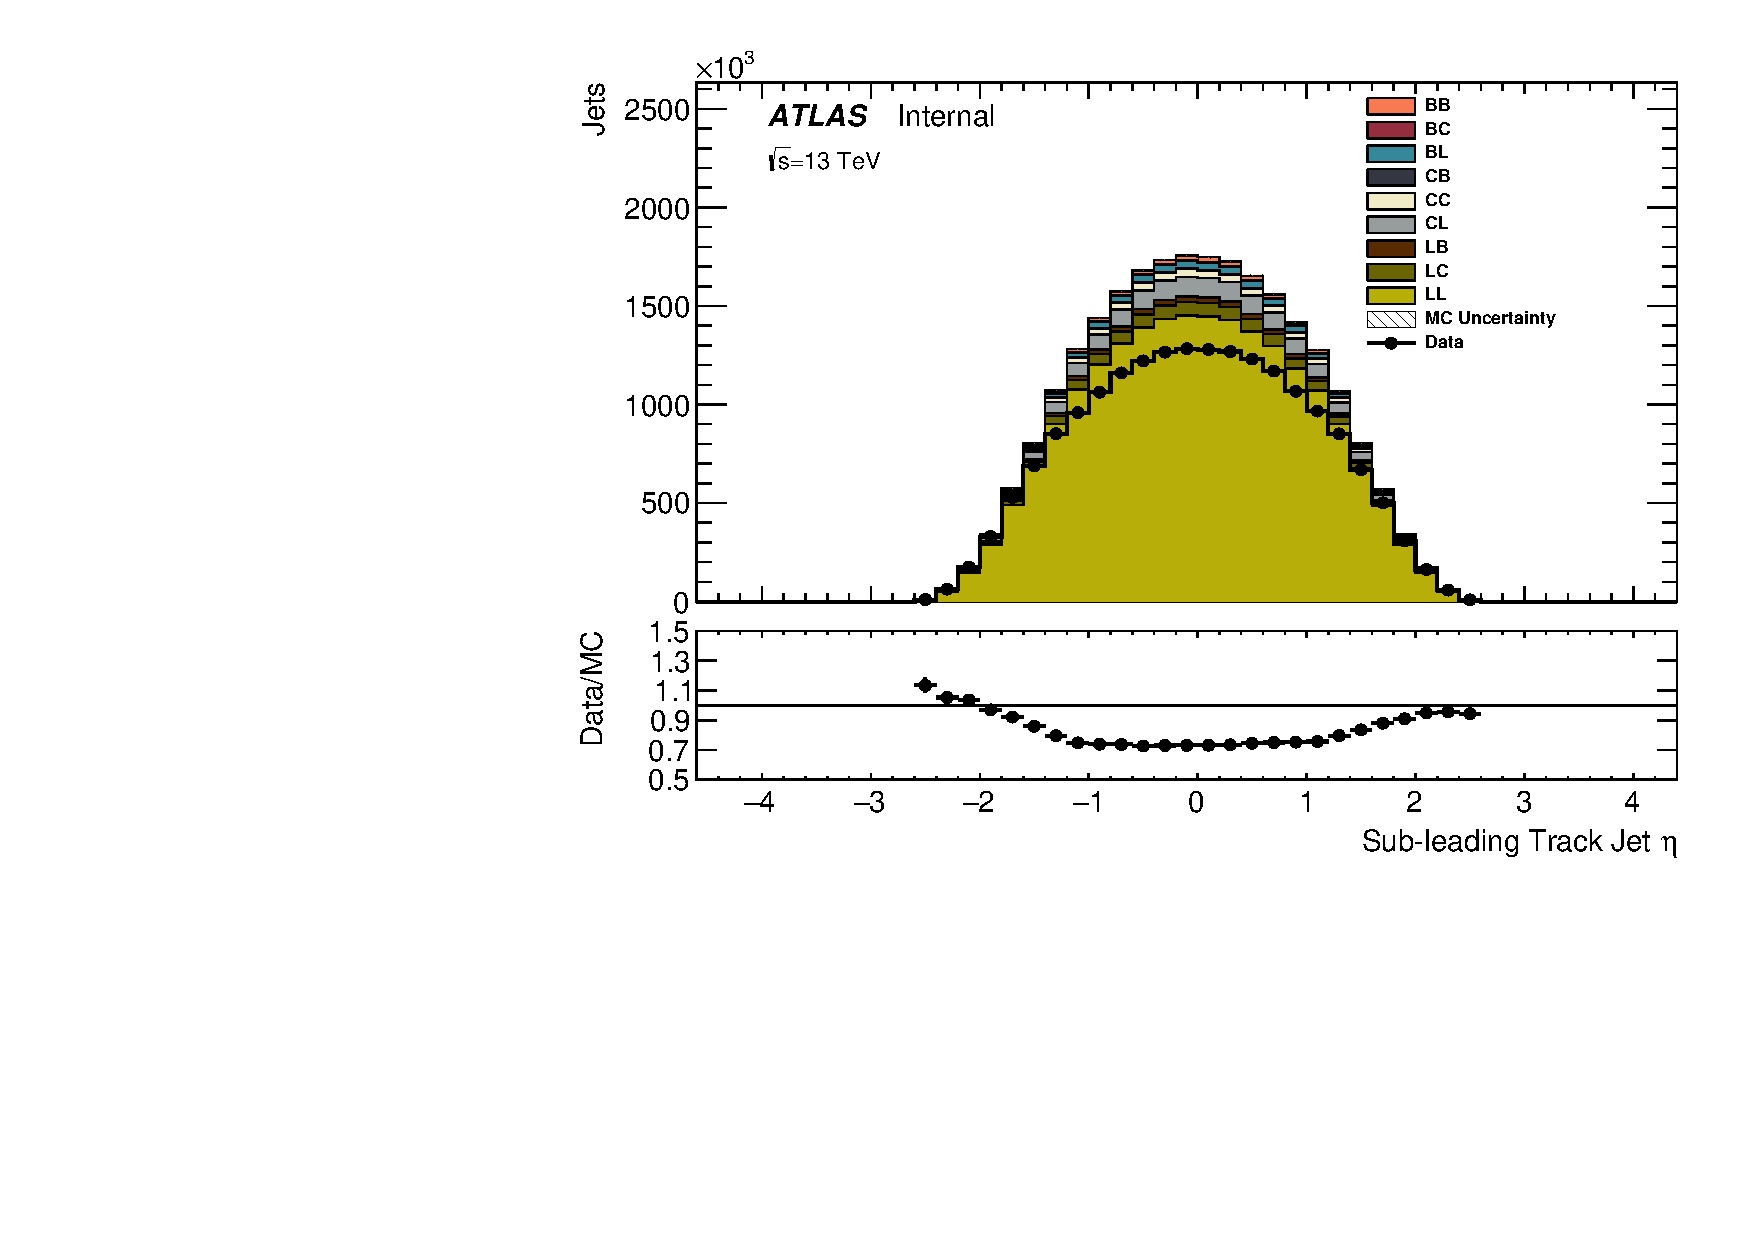
\includegraphics[width=0.45\textwidth]{figures/gbb/SubLeadTrkJet_eta_NoReweight.pdf}
 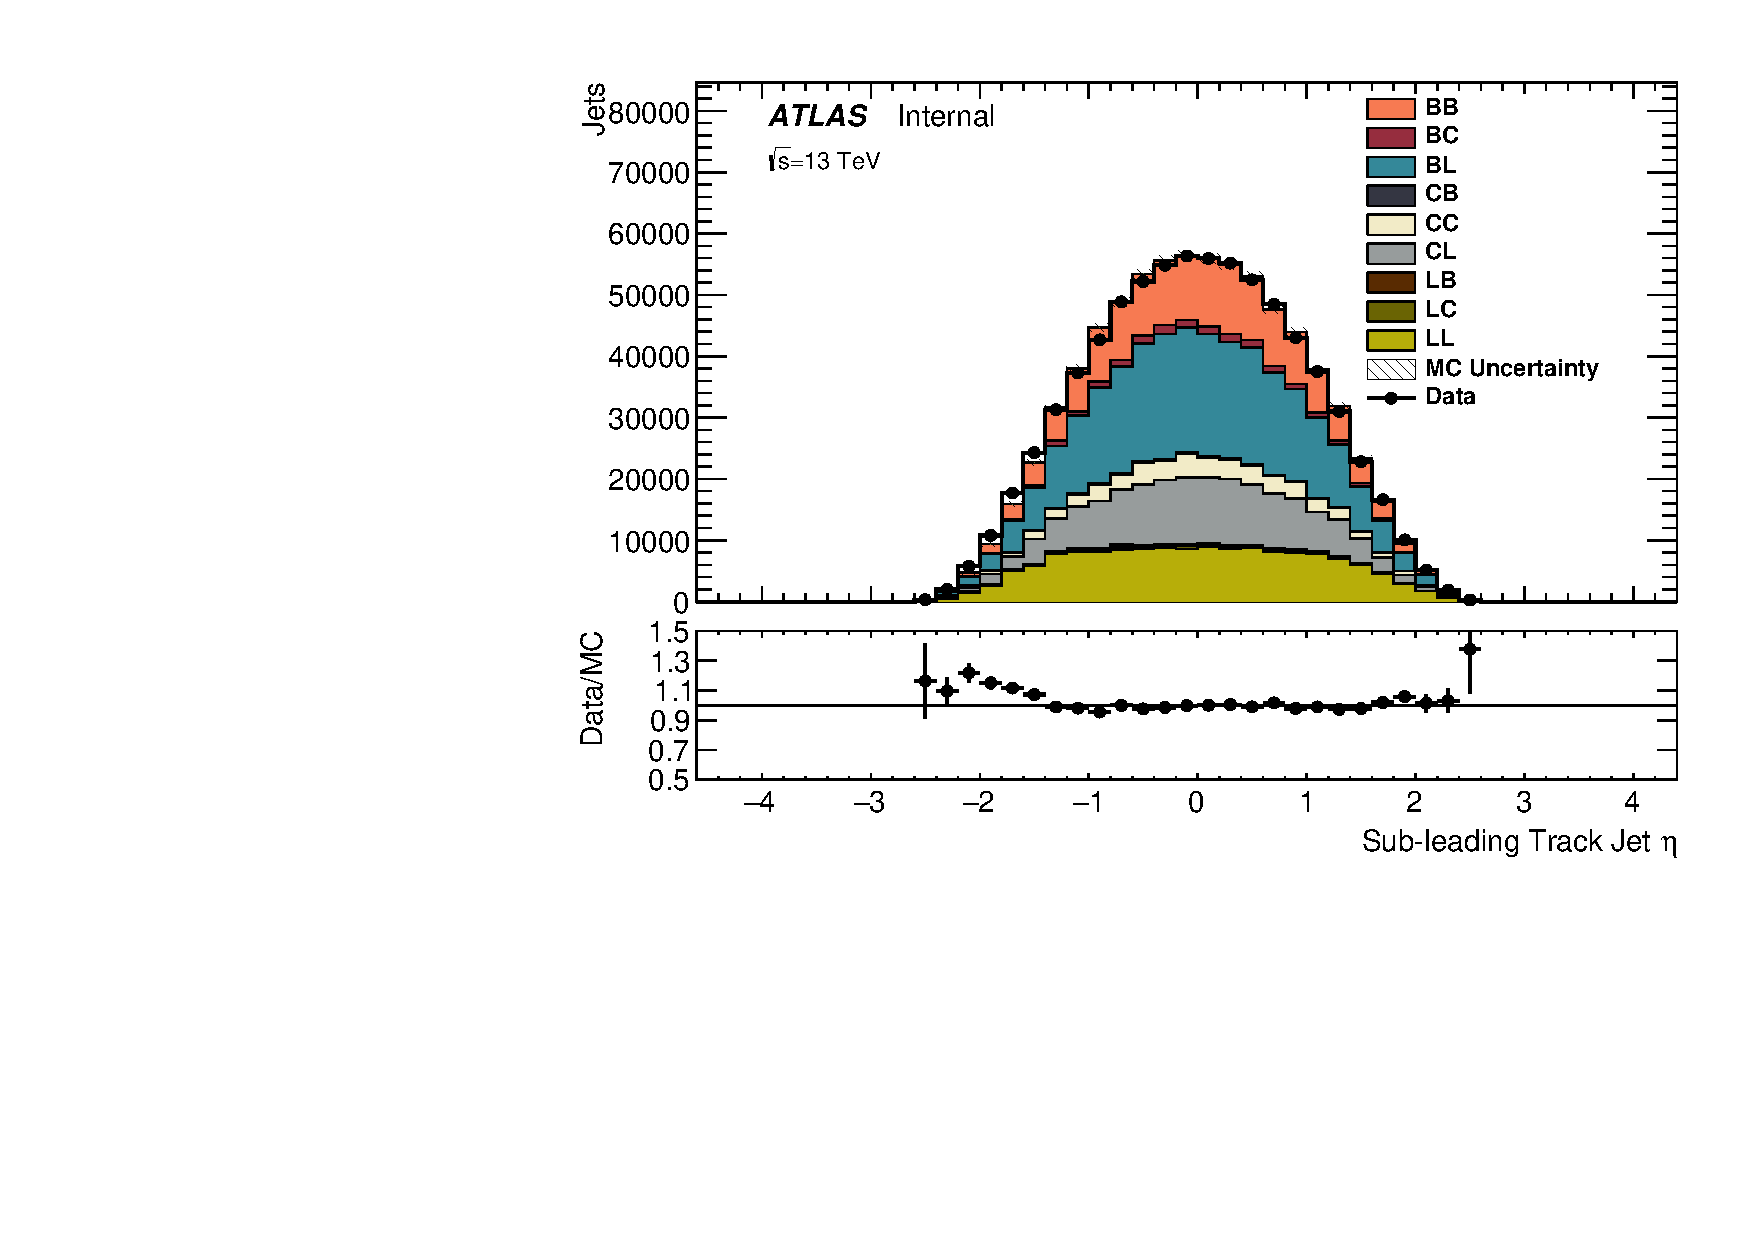
\includegraphics[width=0.45\textwidth]{figures/gbb/SubLeadTrkJet_eta_PreReweight.pdf}\\
 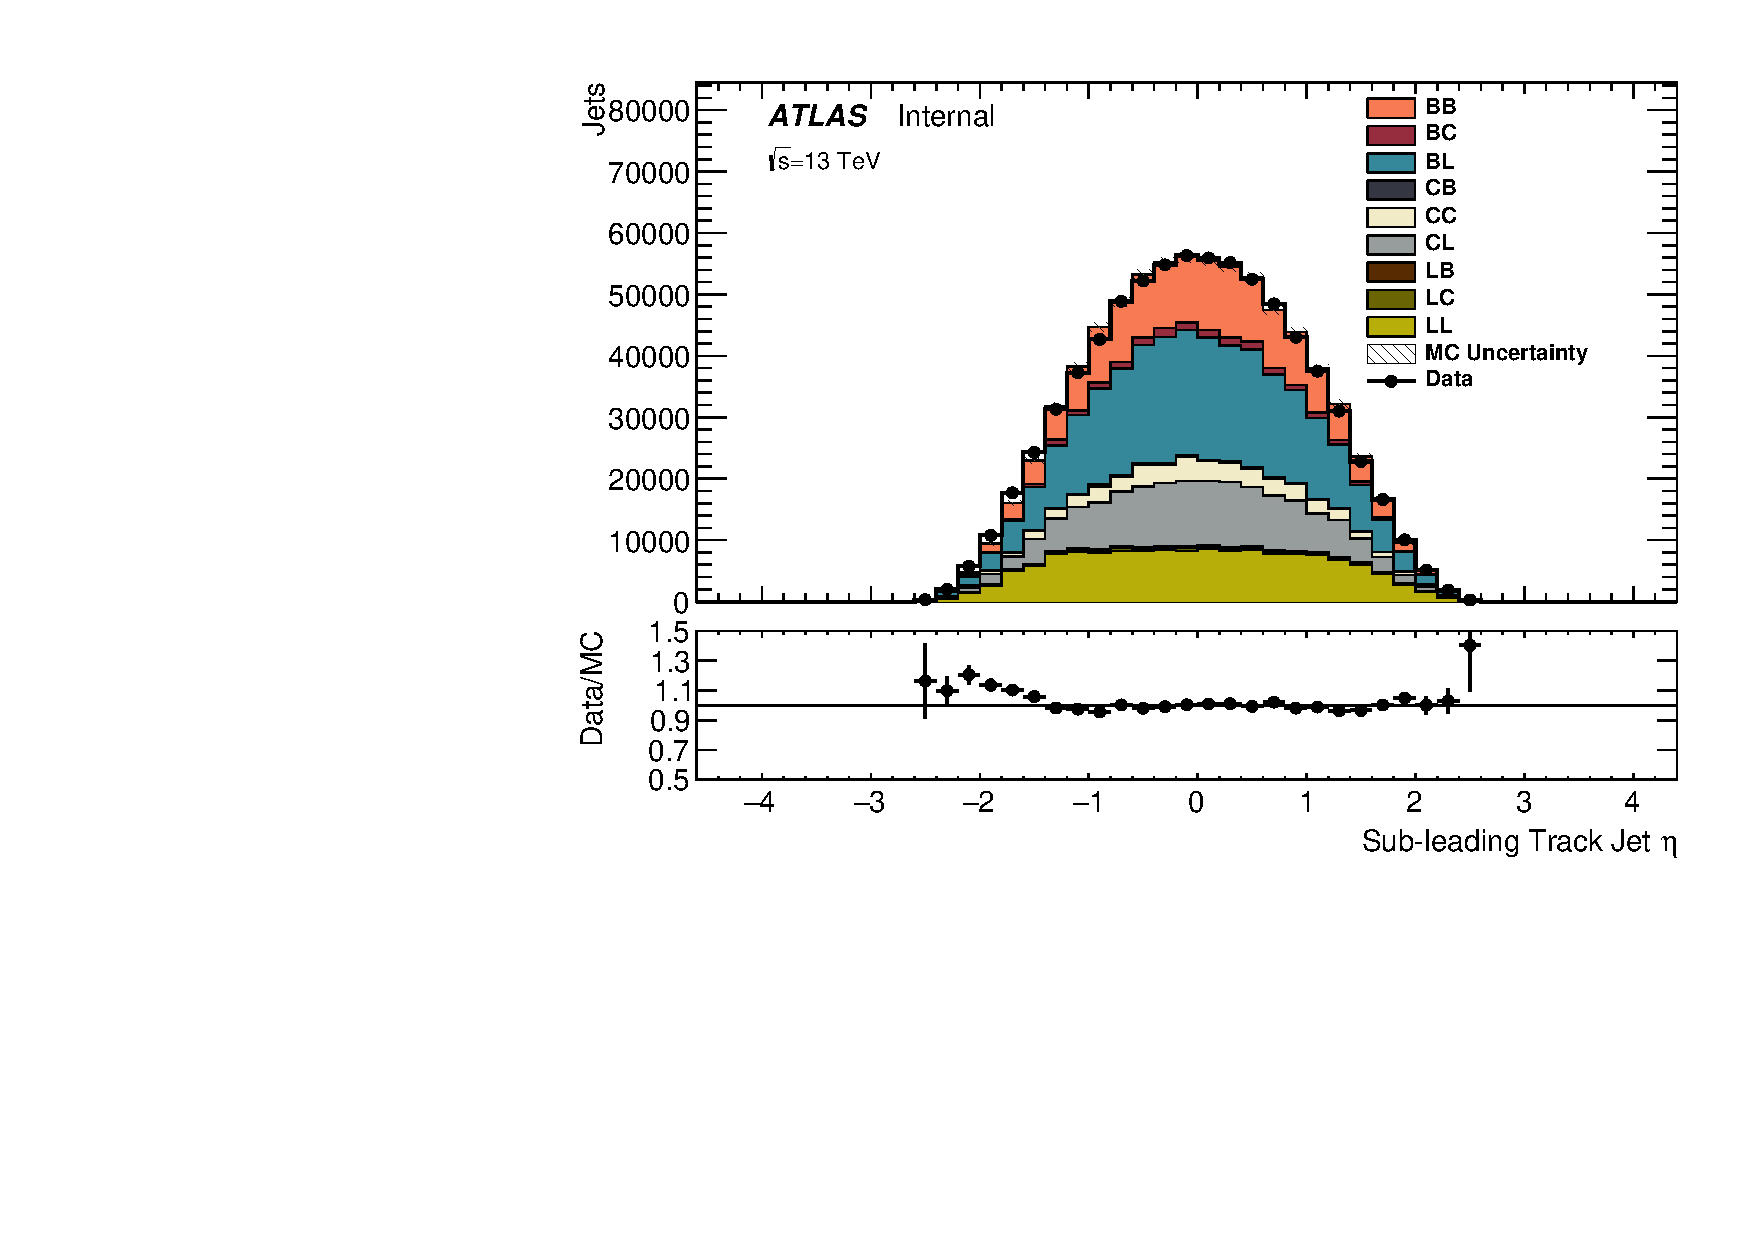
\includegraphics[width=0.45\textwidth]{figures/gbb/SubLeadTrkJet_eta_Reweight.pdf}
\caption{Data/MC comparison of sub-leading track jets $\eta$ before applying $b$-tagging (top left), post $b$-tagging without kinematic reweighting (top right) and post $b$-tagging with kinematic reweighting (bottom). The label of the $R=1.0$ jet flavor content ``XY'' denotes the leading and sub-leading track jet flavor. For example, the flavors of the leading and sub-leading track jet of a ``BL'' $R=1.0$ jet are `B' and `Light' respectively.}
  \label{fig:gbb-eta_subtrkjets}
\end{figure}


